\documentclass{projekt}
\usepackage[none]{hyphenat}
\usepackage{url}
\usepackage[utf8]{inputenc}
\usepackage[T1]{fontenc} 
\usepackage{ae}
\usepackage{fancyhdr}
\usepackage{graphicx}
\usepackage{pdfpages}
\usepackage[all]{xy}
\usepackage{array}
\usepackage[czech]{babel}
\usepackage[activate={true,nocompatibility,all}, stretch=10, shrink=10, step=1, auto=true, draft=false]{microtype}
%\usepackage[total={17cm,28cm}, top=3cm, left=2cm, includefoot]{geometry}
\frenchspacing
\author{Filip Markvart}
\title{Datový model EEG/ERP portálu v prostředcích sémantického webu}
\titlet{} 
\titlett{}
\university{Západočeská univerzita v Plzni}
\faculty{Fakulta aplikovaných věd}
\department{Katedra informatiky a výpočetní techniky}
\subject{Diplomová práce}
\town{Plzeň}
\begin{document}
\pagestyle{fancy}
\renewcommand{\chaptermark}[1]{\markboth{\textit{#1}}{}}
\renewcommand{\sectionmark}[1]{\markright{\textit{#1}}{}}
\cfoot{\thepage}
\lhead{\leftmark}
\rhead{\rightmark}
\maketitle
\chapter*{Prohlášení}
\thispagestyle{empty}
Prohlašuji, že jsem diplomovou práci vypracoval samostatně a výhradně s~použitím citovaných pramenů.
\vskip 1.5em
V Plzni dne \today
\vskip 0.7em
\hskip 9cm Filip Markvart
\chapter*{Abstract}
\thispagestyle{empty}
\hspace{0.65cm}This thesis DODELAT
%describes a transformation of neuroinformatics metadata stored in the relational database to the semantic web standard. The main goal is to investigate existing tools and necessary %modifications that ensure automatic transformation for converting input data. The modified tool is able to process additional semantic information that cannot be stored in the relational %database.


%The last part describes design and implementation of an application that uses annotations to add semantic information to transformed data.

\pagenumbering{gobble} 
\tableofcontents


\pagestyle{fancy}
\renewcommand{\chaptermark}[1]{\markboth{\textit{#1}}{}}
\renewcommand{\sectionmark}[1]{\markright{\textit{#1}}{}}

\cfoot{\thepage}
\lhead{\leftmark}
\rhead{\rightmark}
\parskip 1em
\pagenumbering{arabic} 
\chapter{Úvod}
\hspace{0.65cm}EEG/ERP portál je webová aplikace sloužící výzkumným pracovníkům ke shromažďování a organizaci dat získaných při neuroinformatických experimen-\\tech v EEG laboratoři. Jejím cílem je ukládání naměřených dat v kontextu prováděného experimentu, který lze popsat rozsáhlou množinou různorodých údajů. Tato aplikace již prošla mnohaletým vývojem v jehož průběhu postupně docházelo ke změnám datového modelu kvůli přibývajícím požadavkům na uchovávaná data. Relační databáze jež slouží jako persistentní úložiště tak postupně byla rozšiřována o další tabulky, jejichž počet se k datu tvorby této práce pohybuje v řádu desítek. Většina realizací požadavků na ukládání dalších dat tak přímo znamená zásah nejen do databáze portálu ale také to do datové vrstvy, která ji využívá. V současné době tak databáze obsahuje velké množství tabulek uchovávající různá data, která jsou ale ve smyslu sémantiky často příbuzná a existuje mezi nimi vazba, která je prostřednictvím relačního datového modelu velmi obtížně popsatelná. Zároveň lze očekávat, že budou přibývat požadavky na uchování dalších dat, která navíc nemusejí mít jen homogenní strukturu (ve smyslu relační databáze), ale může se jednat i o množiny sémanticky příbuzných údajů – tzv. metadata, které budou vázány pouze k některým datům. Možnost ukládání strukturně heterogenních, ale sémantický příbuzných metadat je tak dalším otevřeným problémem.

Cílem této práce je prozkoumání struktury a nalezení sémantiky dat v současném datovém modelu relační databáze portálu a následná úprava tohoto modelu do podoby, která by dovolovala uchovat jak sémantiku dat, kterou není možné relačním modelem vyjádřit tak dodávat dynamicky datům přídavná metadata, aniž by muselo docházet k větším zásahům do datového modelu portálu. Pro realizaci úpravy datového modelu budou v této práci využity prostředky tzv. sémantického webu, který poskytuje množství standar-\\dů a technologií pro uchovávání organizaci a správu dat. Tyto technologie a nástroje zde budou popsány a na základě jejich analýzy budou vybrány prostředky, které se využijí pro implementaci úpravy zmiňovaného datového modelu. 
Poslední část práce se věnuje testování modifikovaného modelu a to především z výkonnostního hlediska. Díky této části by mělo být možné posoudit jak užitečnost samotné úpravy tak i použitelnost a efektivnost získaného modelu pro potřeby EEG/ERP portálu.


\chapter{Sémantický web}
\hspace{0.65cm}Dnešní podoba webu, tak jak je všeobecně známa, je tvořena značným množstvím informací, které mají řadu autorů, v podobě různých organizací či jednotlivců, jež se liší jak svým obsahem tak i podobou publikace. Tyto informace jsou poměrně snadno přístupné díky jejich jednoznačné identifikaci prostřednictvím URI identifikátoru (za předpokladu, že jej známe). K usnadně-\\ní získávání dalších (často příbuzných) informací napomáhají tzv. hypertexto-\\vé odkazy, jež usnadňují přístup k dalším zdrojům informací odstraněním požadavku na uživatelovu znalost identifikátoru cílového zdroje. Samotné hypertextové odkazy tak sice zajišťují provázání jednoho informačního zdroje s jiným díky znalosti jeho URI identifikátoru, ale nenesou už žádné další informace, které by například uživateli poskytly další údaje o cílovém zdroji. 
Takováto podoba umožňuje získávání informací jak koncovým uživatelům webu, tak v omezené podobě i vyhledávacím strojům, ale má své limity, neboť se v nepřeberném množství dat lze snadno ztratit, či se jen dostat k irelevantním informacím \cite{_1}.
Základním úkolem sémantického webu, jehož první myšlenky prezentoval v roce 2001 zakladatel konsorcia W3C Tim Berners-Lee, je umožnit aby informace dostupné prostřednictvím webu byly srozumitelné nejen uživatelům, ale také počítačům, jež tato data zpracovávají \cite{_2}. Hlavním cílem je tedy vývoj standardů a technologií, které by umožňovaly přesnější a podrobnější vyhledávání, integraci dat a také automatizaci častých úkonů. 
Sémantický web je založen na několika principech, které budou níže uvedeny.

\begin {itemize}

\item \textbf{Jednoznačná identifikace entit prostřednictvím URI}

\hspace{0.65cm}Veškerá data, reprezentující obvykle objekty reálného světa publiko-\\vaná prostřednictvím webu je možné jednoznačně odkazovat prostředni-\\ctvím identifikátoru URI. Díky této skutečnosti je tak možné realizovat i nepřímé odkazy na objekty, například osobu Petr Novák s emailem petr.novak@w3.org je možné identifikovat jako osobou, jejíž email má URI mailto:petr.novak@w3.org.


\item \textbf{Zdroje i odkazy mezi nimi je možné typovat}

\hspace{0.65cm}Současná podoba webu je tvořena zdroji a odkazy jež je vzájemně propojují. Zdroje, které jsou reprezentovány webovými dokumenty jsou publikovány za účelem poskytnutí informací lidskému uživateli, který dokáže ze samotného obsahu dokumentu získat i některá jeho metadata (pokud jsou v určité formě součástí obsahu) a do jisté míry pak také vztah k ostatním dokumentům, na něž vedou případné odkazy. Stroje v podobě různých vyhledávačů či automatů pro shromažďování dat ale tuto schopnost nemají nebo je pro ně příliš náročná. Řešením sémantického webu je typování jak samotných zdrojů, tak i odkazů, které je provazují. Díky této skutečnosti je pak možné webovým doku-\\mentům dodávat metadata jako např. autora, verzi či závislost na jiném dokumentu. Z hlediska typování odkazů je například možné jeden webový zdroj označit pouze jako odlišnou verzi jiného zdroje.


\item \textbf{Tolerance neúplných informací}

\hspace{0.65cm}U současně podoby webu může nastat situace, kdy některý zdroj není dostupný. V takovém případě uživatel ztrácí přistup k danému dokumentu, ale díky koncepci webu není nikterak ohrožena dostupnost ostatních zdrojů. V případě sémantického webu se situace nemění, nedostupnost některého zdroje není žádnou překážkou, neboť nástroje sémantického webu zpracovávají pouze ty informace, které jsou dostupné a z těch vytvářejí závěry. V důsledku je tak možné dojít při zpracovávání dat ke stejným výsledkům, jako v případě, když jsou zpracovávány jen některé vybrané informace, jejichž rozsah je explicitně definován.

\item \textbf{Zpracování neověřených dat}

\hspace{0.65cm}Při zpracovávání informací pocházejících z neověřených zdrojů je možné dohledávat prostřednictvím typovaných odkazů důvěryhodná data, jejichž obsah a odkazy poslouží jako ověřovací prostředek. Tento princip je možné uvést na následujícím příkladu. Aplikace zpracovávající data sémantického webu vyhledá informace, přičemž je kladen požadavek na vysokou pravděpodobnost správnosti výsledku. Pokud některá část nalezených informací pochází z neověřeného zdroje, je možné vyhledávat například jejich autora v odkazech zdrojů, které jsou důvěryhodné či ověřené. V případě úspěchu nalezení takového odkazu u více různých zdrojů je pak možné považovat zkoumaný zdroj s vysokou pravděpodob-\\ností rovněž za důvěryhodný a tím zajistit plnění požadavků na výsledek.

\item \textbf{Podpora paralelního vývoje dat}

\hspace{0.65cm}V průběhu času nezřídka nastávají situace, kdy autoři, či skupiny autorů publikují obdobná data na různých místech nebo v odlišném čase. Obsah těchto dokumentů se může navíc lišit svým jazykem či použitou terminologií, ač význam bude shodný. S využitím prostředků sémantického webu je ale možné prostřednictvím typovaných odkazů zajistit provázanost významově obdobných či na sebe navazujících dat i přes překážku rozdílnosti jejich podoby zápisu. Navíc je také možné dodávat nové informace bez nutnosti úpravy původních dat, která tím pádem nezmění svoji strukturu \cite{_1}.

\end{itemize}


\section{Architektura sémantického webu}
\hspace{0.65cm}Architektura sémantického webu sestává z více oddělených vrstev, mezi nimiž je zajištěna zpětná i dopředná kompatibilita \cite{_3}. Nejnižší vrstva je tvořena dvěma technologickými standardy – URI identifikátory sloužící pro jednoznačné pojmenování zdrojů dat a Unicode kódování mezinárodní znako-\\vou sadou. Druhou vrstvu architektury, jež je patrná z obrázku 2.1, reprezentu-\\je značkovací jazyk XML (Extensible Markup Language), který umožňuje tvorbu strukturovaného dokumentu za užití vlastních značek. Tato vrstva zároveň zajišťuje definici XML schématu včetně jmenných prostorů. RDF + rdfschema jež následuje je klíčovou vrstvou sémantického webu neboť dovoluje tvorbu vazeb a vztahů mezi jednotlivými zdroji, které jsou typované spolu s odkazy. Je tak možné definovat libovolné vztahy mezi objekty či jejich kategoriemi bez nutnosti specifikace významu samotných vazeb či objektů. Díky RDF schématu je vytvářena základní sémantika datového modelu, která už definuje význam některých elementů jako třídy či podtřídy. 
Vrstva ontologického slovníku, zastoupená jazykem OWL, nabízí pokročilou reprezentaci znalostí na úrovni deskripční logiky a umožňuje tak vytvářet složitější struktury sloužící k popisu různých vlastností objektů \cite{_2}. Poslední vrstvou, která je jako všechny předchozí zmíněné konsorciem W3C standardizo-\\vaná jsou digitální podpisy. Ty poskytují možnosti například pro detekci různých verzí dokumentů. Zbylé výše znázorněné vrstvy slouží pro definice a vyhodnocování odvozovacích pravidel a v současnosti jsou ve fázi vývoje \cite{_1}.

\begin{figure}[htb]
\begin{center}
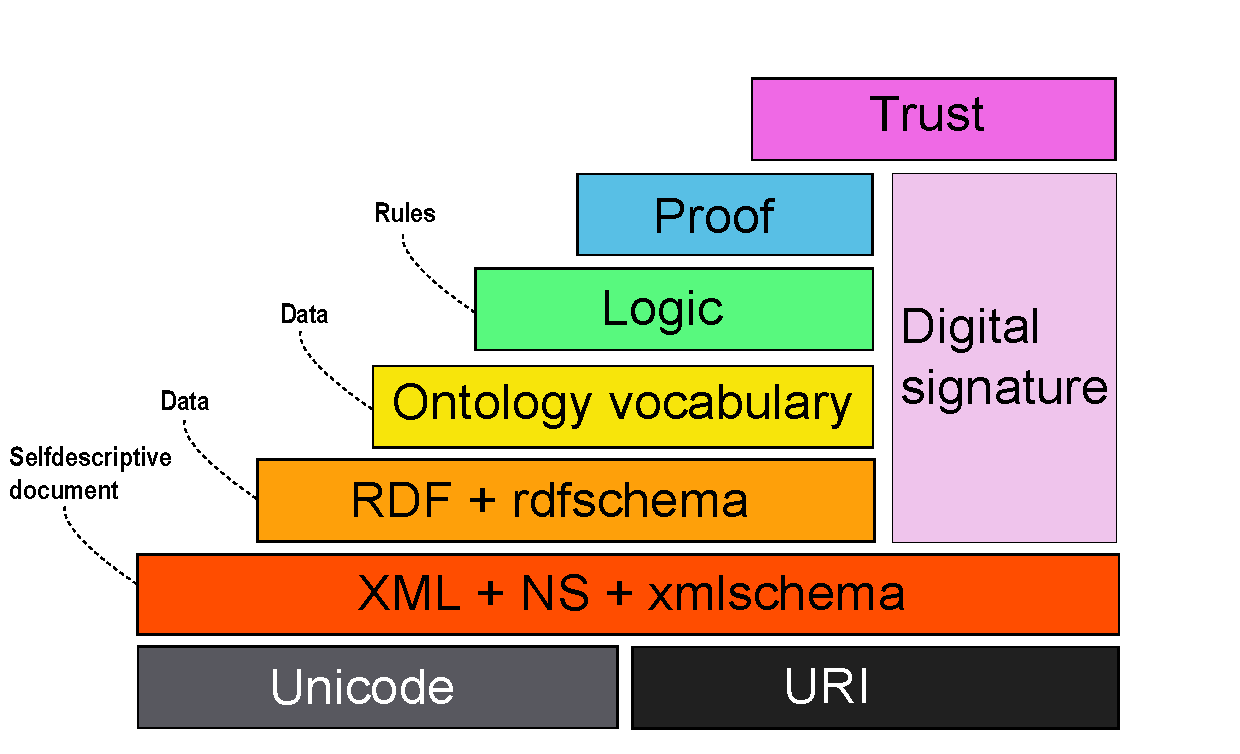
\includegraphics[scale=0.62]{architektura.pdf}
\caption{Architektura sémantickém webu \cite{_1}}
\end{center}
\end{figure}

Vrstvení jazyků sémantického webu je podstatné pro úroveň expresivity znalostního modelu, neboť s rostoucí vyjadřovací možností jazyka také roste složitost dotazovacích operací nad modelem. Je tedy nutné před započetím tvorby modelu nejprve zjistit jeho požadovanou expresivitu a podle té zvolit pro zápis dat jazyk, který ji dovoluje obsáhnout. Využívá se tedy skutečnosti, že jazyk vyšší vrstvy zahrnuje vyjadřovací schopnosti vrstev nižších\cite{_2}. 
Další podkapitoly se budou zabývat podrobněji jednotlivý zmíněnými technologiemi.

\section{XML}
\hspace{0.65cm}XML (eXtensible Markup Language) je značkovací jazyk sloužící pro popis hierarchických struktur textových dokumentů prostřednictvím tzv. tagů. Tag je konstrukce, která slouží k počátečnímu a koncovému ohraničení společně definovaného elementu. Tag lze chápat jako prostředek pro dodání metadat ke textové struktuře, jež ohraničuje. Příkladem může být následující zápis {\it <prijmeni>Novák</prijmeni>}, kde elementu {\it Novák} je dodána meta informace, že se jedná o příjmení. Samotné XML ale nedefinuje žádný sémantický význam tagů, slouží pouze pro specifikaci syntaxe na úrovní XML dokumentu. Pro definici (zejména hierarchické) struktury XML dokumentu slouží XML Schema, které umožňuje zápis pravidel, jež musí cílový dokument dodržovat pro zachování své validity. Ze strany sémantického webu ale nemají pravidla XML Schema žádný sémantický význam a slouží tak pouze pro definici struktury a syntaxe. Zmíněné schéma také definuje základní datové typy (čísla, řetězce, čas a pod.), které nabývají významu v sémantických jazycích jako je RDF \cite{_3}.


\section{RDF}
\hspace{0.65cm}Technologický základ sémantického webu tvoří jazyk RDF (Resource Description Framework), jež slouží jako obecný rámec pro popis, výměnu a opětovné použití metadat \cite{_3}. Tento rámec poskytuje jednoduchý model sloužící pro popis zdrojů jež je nezávislý na jeho konkrétní implementaci \cite{_4}. Samotné informace o objektu jsou realizovány prostřednictvím tvrzení, jež se označují jako trojice (anglicky triple). Každou trojici tvoří spolu subjekt, predikát a objekt. Subjekt je libovolný objekt identifikovatelný prostřednictvím URI, který se snažíme prostřednictvím trojice popisovat, zaznamenat nějakou jeho vlastnost. Tato vlastnost se popisuje prostřednictvím predikátu, který vede ve směru od subjektu ke objektu, přiřazuje tedy subjektu nějaký objekt prostřednictvím této vlastnosti. Cílový objekt pak představuje hodnotu, které předchozí objekt nabývá pro daný predikát. 
Tento princip je možné znázornit na jednoduchém tvrzení, zapsaném větou „Martin staví dům.“ Subjektem trojice potom bude Martin, predikátem staví a objektem dům, tak jak je znázorněno na obrázku 2.2. 
\\
\vspace{0.1cm}

\begin{figure}[htb]
\begin{center}
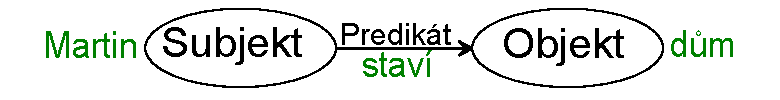
\includegraphics[scale=0.9]{trojice.pdf}
\caption{Příklad RDF trojice}
\end{center}
\end{figure}

Dle definovaného standardu \cite{_5} je možné, aby objektem byl jiný subjekt. Díky této skutečnosti je možné jednotlivé trojice spojovat do většího celku, který ve výsledku tvoří strukturu orientovaného grafu, kterou lze označit jako model \cite{_3}. Jednoduchým model tvořený dvěma trojicemi lze vytvořit využitím dalšího tvrzení „Dům stojí v Plzni.“ V předchozí trojici pak bude dům subjektem namísto objektu a dojde tak ke spojení dvou trojic (za předpokladu že v obou tvrzeních je myšlen stejný fyzický dům), tak jak je znázorněno na obrázku 2.3. 

\begin{figure}[htb]
\begin{center}
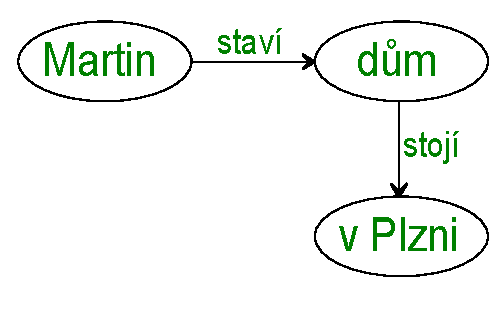
\includegraphics[scale=0.9]{miniStrom.pdf}
\caption{Příklad jednoduchého RDF modelu}
\end{center}
\end{figure}


Z hlediska implementace mohou být uzly orientovaného grafu datového modelu tvořeny URI identifikátorem, anonymním listem nebo literálem \cite{_6}. URI identifikátor obsahuje pouze adresu zdroje v textové podobě ve znakové sadě Unicode a zastupuje tak konkrétní jedinečný objekt. Anonymní list (anglicky blank node) je prvek nahrazující URI identifikátor při absenci unikátní adresy zdroje. Tato entita přestavuje zdroj, který je sice v rámci grafu popisován prostřednictvím trojic, ale není potřeba (často z hlediska významu), aby byl dostupný i vně grafu. S URI má společné to, že musí nést adresu zdroje (její syntaxe není implicitně definována), ale liší se skutečností, že tato adresa musí být unikátní pouze v rámci obalujícího modelu, nikoliv vně grafu. Může tak nastat situace, že dva odlišné modely budou obsahovat (ze syntaktického hlediska) dva stejné anonymní uzly, což v případě URI možné není (při respektování specifikace). Tento list tak může představovat anonymní objekt sloužící ke vytvoření vazby mezi jinými objekty, které jsou z hlediska sémantiky významné \cite{_5}. Jako příklad je možno uvést následující tvrzení. „Martinův přítel zná předpověď počasí. Počasí bude deštivé.” Zjednodušeným převodem předchozích vět na trojice v podobě subjekt – predikát – objekt získáme: {\it Martin – má – přítel}, {\it přítel – zná – počasí},  {\it počasí – bude – deštivé.} 
Subjekt resp. objekt přítel zde může být reprezentován anonymním listem, v případě že jedinou signifikantní informací (z vnějšího pohledu na datový model) je Martinova získaná znalost počasí, nikoliv už jeho přítel, jež mu ji zprostředkoval. 
Poslední možnou reprezentací entity trojice je literál, jež nese Unicode textový řetězec, který slouží pro zápis koncové informace (užitečné pro lidského čtenáře). Literál může také navíc obsahovat položku, pro označení jazyka, ve kterém je textová informace zapsána \cite{_6}. 
\\
\\
Pro komponenty každé trojice grafu platí následující pravidla \cite{_6}.

\begin {itemize}

\item \textbf{subjekt} - může být tvořen URI identifikátorem nebo anonymním listem
\item \textbf{predikát} - může být tvořen pouze URI identifikátorem
\item \textbf{objekt} - může být tvořen URI, anonymním listem nebo literálem

\end{itemize}


Pro zápis trojic RDF grafu je sice možné využít grafické podoby, ale pro vyjádření sémantiky webových zdrojů je nejvhodnější využít syntaxe jazyka XML. Níže uvedená ukázka kódu reprezentuje XML zápis trojice z obrázku 2.2.

\begin{verbatim}
<rdf:RDF xmlns:rdf="http://www.w3.org/1999/02/22-rdf-syntax-ns#"
         xmlns:dc="http://purl.org/dc/elements/1.1/">
  <rdf:Description rdf:about="http://www.w3.org/Person/Martin">
    <dc:stavi>dům</dc:stavi>
  </rdf:Description>
</rdf:RDF>

\end{verbatim}

Samotné RDF nedefinuje trojicím ani jejím částem sémantiku, ale dovoluje vyjádřit základní vztahy náležitosti prvků do kategorie prostřednictvím kontej-\\nerů a kolekcí (např. rdf:Bag, rdf:List) \cite{_2}. Pro dodání základní sémantiky slouží schéma popsané v následující podkapitole.

\section{RDFS}
\hspace{0.65cm}RDF Schema (Resource Description Framework Schema) funguje jako základní jazyk pro tvorbu ontologií s velmi jednoduchou sémantikou. Toto schéma rozšiřuje jazyk RDF o možnosti vyjádření vlastností objektů, konstruk-\\ce tříd objektů a popis jejich hierarchie \cite{_2}. 
Prostředky jazyka RDFS umožňují především vyjádření vztahů mezi zdroji, které lze rozdělit na dvě skupiny – třídy a vlastnosti.

\subsection{Třídy}
\hspace{0.65cm}Skupiny zdrojů je možné rozčleňovat do skupin označovaných jako třídy (classes), jejichž členové se nazývají instance třídy. Na úrovni RDFS se rozlišují třídy od svých instancí a každá třída jich může mít neomezený počet. Dvě třídy mohou mít navíc shodnou množinu instancí tříd a zároveň tyto třídy mohou být navzájem různé. Bude-li se tedy například definovat třída {\it A} jako osoby pracující v kanceláři {\it 1} a třída {\it B} jako osoby žijící ve městě {\it X}. Potom je možné aby různé třídy {\it A} a {\it B} měly stejné množiny instancí, za předpokladu, že každá osoba pracující v kanceláři {\it 1} bydlí ve městě {\it X}. Pro třídy platí také dědičnost – bude li třída {\it B} podtřídou {\it A}, pak všechny instance {\it B} jsou zároveň instancí třídy {\it A}. Koncept tříd RDFS definuje následující konstrukce \cite{_7}:

\begin {itemize}

\item \textbf{rdfs:Resource} představuje RDF zdroj, který je obalující třídou všech prvků – je tedy nejvýše postavenou rodičovskou třídou, {\it rdfs:Resource} je zároveň instancí {\it rdfs:Class}
\item \textbf{rdfs:Class} reprezentuje rodičovskou třídu všech RDF tříd zdrojů, čímž je {\it rdfs:Class} instancí {\it rdfs:Class} (sebe sama)
\item \textbf{rdfs:Literal} třída je instancí {\it rdfs:Class}, která slouží pro reprezentaci RDF literálů a je podtřídou {\it rdfs:Resource}
\item \textbf{rdfs:Datatype} je obalující třídou pro datové typy, které jsou její instancí, {\it rdfs:Datatype} je zároveň podtřídou i instancí {\it rdfs:Class} a každá její instance je podtřídou {\it rdfs:Literal}
\item \textbf{rdf:XMLLiteral} je třída XML literálů, která je podtřídou {\it rdfs:Literal} a instancí {\it rdfs:Datatype}
\item \textbf{rdf:Property} představuje rodičovskou třídu všech definovaných vlastností a je instancí {\it rdfs:Class}


\end{itemize}


\subsection{Vlastnosti}
\hspace{0.65cm}Vlastnosti (properties) slouží k vyjádření vztahu mezi dvěma zdroji – na úrovni trojice mezi subjektem a objektem. Koncept RDFS definuje následující vlastnosti:

\begin {itemize}


\item \textbf{rdfs:range} je instancí {\it rdf:Property}, která slouží ke vyjádření, že objekt jehož predikát má definovaný {\it  rdfs:Range X} bude zároveň instancí {\it X}, například z následujících trojic {\it A – rdfs:Range B a X – A – C} bude vyplývat, že {\it C} je instancí {\it B}, 
zároveň platí, že objekt s definovaným predikátem může být instancí více tříd (pokud má predikát definováno více {\it  rdfs:Range}).

\item \textbf{rdfs:domain} představuje instanci {\it rdf:Property}, která vyjadřuje, že zdroj (subjekt) jehož predikát má definovaný {\it rdfs:Domain X} bude také instancí {\it X}, tento zdroj může být jako v předchozím případě instancí více tříd při definování více {\it rdfs:Domain}
\item \textbf{rdf:type} slouží k definování, že zdroj (subjekt) je instancí třídy definované objektem, pokud tedy platí {\it A rdf:type B}, pak {\it A} je instancí {\it B}
\item \textbf{rdfs:subClassOf} je vlastnost sloužící k vyjádření náležitosti instancí jedné třídy jako instancí jiné třídy, pokud platí {\it A rdfs:subClassOf B}, pak {\it A} je podtřídou {\it B} a všechny instance třídy {\it A} jsou zároveň instancí třídy {\it B}, tato vlastnost je navíc tranzitivní, takže popsanou dědičnost je možné řetězit do libovolné délky
\item \textbf{rdfs:subPropertyOf} slouží k vyjádření dědičnosti vlastností, pokud platí {\it P1 subproperty P2}, pak pro trojici {\it A P1 B} platí, že subjekt {\it A} má pro vlastnost {\it P1} i {\it P2} pro objekt {\it B}
\item \textbf{rdfs:label} umožňuje zdroji (subjektu) přidat textovou informaci jako lidsky čitelnou náhradu pro označení zdroje
\item \textbf{rdfs:comment} dovoluje přidat zdroji popisek, který usnadňuje lidskému uživateli pochopit význam zdroje \cite{_7}

\end{itemize}

Vyjádření vztahů mezi jednotlivými vlastnostmi a třídami je patrné z obrázku 2.4. Rámec RDFS dále ještě definuje vlastnosti a třídy pro kontejnery a kolekce, které je možné naleznout ve \cite{_7}.

\begin{figure}[htb]
\begin{center}
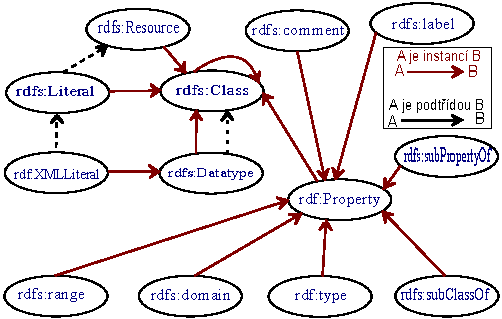
\includegraphics[scale=1.4]{rdfs.pdf}
\caption{Vztahy mezi vlastnosmi a třídami RDFS}
\end{center}
\end{figure}

\section{Ontologie}
\hspace{0.65cm}Znalostní modely, jež jsou popisované vyššími jazyky sémantického webu se označují jako ontologie. Ontologie ovšem není pouze abstraktním znalostním modelem, ale slouží i jako prostředek k získání interoperability, tedy schopnosti vzájemné spolupráce oddělených systémů na úrovni sdílení dat a poskytování služeb \cite{_2}. Definicí ontologie v informatice kterou uvádí Thomas Gruber, zakladatel ontologického inženýrství, je „formální specifikace sdílené konceptu-\\alizace“\cite{_8}. V této definici je formálností myšleno vyjádření znalostí prostřed-\\nictvím jazyka s formálním a logickým základem. Pojem konceptualizace znamená definování konceptů na dané úrovni abstrakce, jež odpovídá požadav-\\kům pro model domény. Tuto doménu pak vytvářejí osoby, pro které je daná ontologie závazně (vzájemnou dohodou) definovaná jako prostředek pro popis dat, jež musejí všichni členové dodržovat \cite{_2}. V důsledku se tak jedná o tvorbu abstraktního modelu v určené oblasti, kde se definují pojmy společně se vzájemný vztahy vyjádřené logickým jazykem. Cílem explicitní specifikace pojmů a vztahů je snaha o porozumění znalostně orientovaných systémů \cite{_9}.
Ontologie lze z hlediska vývoje rozčlenit do tří kategorií:

\begin {itemize}

\item \textbf{Terminologické (lexikální)} Slouží především ke zachycení taxonomie definovaných pojmů a popisu jejich vzájemných vztahů. Jejich realizace se často podobá slovníkům synonym.
\item \textbf{Informační} Zastávají roli služby stojící nad databází, která zajišťuje vyšší míru abstraktnosti při databázovém dotazování.
\item \textbf{Znalostní} Dovolují reprezentaci znalostí především v oblasti umělé inteligence, kde jsou chápány jako logické teorie, jejichž elementární prvky se definují prostřednictvím formálního jazyka. Využívají se zej-\\ména ve znalostně orientovaných systémech \cite{_10}.

\end{itemize}

Dle míry formalizace a cílového předmětu konceptualizace se rozlišují 4 kategorie ontologie.

\begin {itemize}

\item \textbf{Doménové} Zabývají se specifikací určité oblasti – domény.
\item \textbf{Generické} Blíží se svou podobou doménovým, ale pokrývají širší množinu dat a zachycují tak obecnější koncepty, nejdou ovšem do příliš velké hloubky. Popisují například realitu prostřednictvím vzájemných časoprostorových pozic objektů. Často se snaží zachytit všeobecné zna-\\losti, které odpovídají běžně používaným lidským vědomostem.
\item \textbf{Úlohové} Tyto ontologie jsou zaměřené zejména na odvozovací procesy namísto záznamu znalostí a slouží především jako modely pro řešení určitých problémů – např. pro diagnostiku či plánování.
\item \textbf{Aplikační} Jsou většinou vázány na specifické aplikace, kde spojují doménovou a úlohovou ontologii \cite{_10}.
\end{itemize}

Pro realizaci popsaných ontologií je zapotřebí jazyka, který by dovoloval formální zápis. Výše uvedené schéma RDFS je z hlediska sémantického webu základní podobou ontologie, kterou je dále možné rozšiřovat například využi-\\tím jazyků jako je OWL.


\section{OWL}
\hspace{0.65cm}OWL (Web Ontology Language) je jazyk sémantického webu navržený pro získávání a zpracování informací prostřednictvím strojů (aplikací), namísto současného stavu, kdy jsou informace určeny pouze pro lidské uživatele. Tento jazyk využívá technologií XML, RDF a RDFS jakožto primárních prostředků pro tvorbu ontologických slovníků se základní sémantikou, kterou sám dále rozšiřuje o možnosti vyjádření složitějších výrazů a jejich vzájemných vztahů \cite{_11}. Mezi tato rozšíření patří například kardinalita, univerzální a existenční kvantifikace, matematické charakteristiky vlastností jako např. tranzitivnost, disjunktnost či inverze a anonymní třídy (sloužící  často k jednorázovému využití) \cite{_12}.
Vzhledem k tomu, že OWL nabízí poměrně pokročilou úroveň expresivity jazyka, je nutné brát v potaz výpočetní složitost algoritmů odvozo-\\vacích a usuzovacích nástrojů pracujících s vytvořenou ontologií. Z tohoto důvodu jsou specifikovány 3 varianty jazyka OWL, které se vzájemně liší mírou expresivity \cite{_2}.


\begin {itemize}

\item \textbf{OWL Lite} Umožňuje definovat hierarchický systém tříd s jednoduchými omezeními vazeb \cite{_11}. Dále poskytuje prostředky pro zaznamenání symetrické, transitivní a inverzní vlastnosti a také jednoduchá omezení na velikosti množin vybraných objektů modelu – kardinalitu, která je ale v této verzi omezena pouze na přípustné hodnoty 0 a 1 \cite{_2}.
\item \textbf{OWL-DL} Tato varianta poskytuje maximální možnou expresivitu jazyka, u které je stále splněna podmínka rozhodovací úplnosti (jakékoliv rozhodovací pravidlo je možné použít na kteroukoliv část ontologie) a výpočetní splnitelnosti (veškeré výsledky odvozovacích operací budou získány v konečném čase) \cite{_2}. OWL-DL nabízí veškeré konstrukce jazyka OWL, které ale podléhají určitým omezením při jejich použití, např. není možné využít omezení kardinality pro vlastnosti definované jako tranzitivní. Z hlediska množiny dostupných jazykových konstrukcí dovoluje tato varianta oproti OWL Lite definovat navíc sjednocení, disjunkce a doplňky tříd nebo libovolné omezení kardinality \cite{_11}.
\item \textbf{OWL-Full} Je variantou, která poskytuje maximální možnou expresivitu, ke které využívá stejně jako předchozí verze všech konstruktů jazyka OWL. Tato varianta neklade žádná omezení pro vyhodnocovací pravidla, díky čemuž ale není možné zaručit výpočetní splnitelnost. OWL-Full dovoluje ještě navíc uživatelskou změnu sémantického významu nativně definovaných konstrukcí jazyků RDF a OWL. Tato verze ovšem není prakticky příliš využitelná, neboť v současnosti nejsou známé žádné efektivní algoritmy, které by dovolovaly nad modelem dat provádět usuzovací operace využívající všech vlastností OWL-Full \cite{_2}.

\end {itemize}

Každá verze OWL je rozšířením svého předchůdce díky čemuž je ontologie vyjádřená v jednodušší variantě platná i pro verzi vyšší, např. tedy každá ontologie zapsaná ve OWL Lite bude plně validní ve OWL-DL (což ale obráceně neplatí) \cite{_11}.
Mezi typické odvozovací úlohy v kontextu OWL patří například odvozování taxonomické struktury, ověřování příslušnosti instance ke třídě, klasifikace individuí vzhledem k definované ontologii či testování splnitelnost logické teorie \cite{_12}.


\section{SPARQL}
\hspace{0.65cm}Základním prostředkem pro dotazování nad daty sémantického webu je jazyk SPARQL (SPARQL Protocol and RDF Query Language). Tento jazyk standardizovaný konsorciem W3C umožňuje vytvářet dotazy nad RDF grafy prostřednictvím vzorů RDF trojic spolu s logickými operacemi konjunkce a disjunkce \cite{_2}. Konstrukce těchto dotazů je sice složitější než v případě SQL dotazů nad relačními databázemi, ale umožňuje ze zdrojové ontologie získávat komplexnější informace \cite{_3}. SPARQL dotaz se skládá ze 3 základních částí. První část – označovaná jako prolog slouží k definování jmenných prostorů a prefixů, které budou v dalších částech dotazu použity. Druhou částí je hlavička dotazu, kde se určuje jaký typ dotazu se bude v další části provádět. Třetí a hlavní část SPARQL slouží k definování cílové ontologie (RDF grafu) pro dotazování (v případě, že cílový graf je implicitně definován, je tato část vynechána) a proměnných včetně samotných vyhledávacích podmínek v podobě grafových vzorů (graph pattern)\cite{_2}.
Tento jazyk částečně vychází ze SQL, což je patrné i na jeho syntaxi. Např. klauzule FROM slouží pro výběr cílového grafu pro dotazování, či klíčové slovo WHERE slouží pro uvození zápisu souboru RDF trojic – tzv. grafového vzorce, jež je jádrem dotazu. Vyhodnocování dotazu poté probíhá takovým způsobem, že dochází k porovnávání grafového vzorce se s RDF daty \cite{_13}. 
Pro názornost je níže uveden zápis jednoduchého SPARQL dotazu, který slouží k vyhledání jmen a příjmení všech osob v implicitně zadaném grafu.

\begin{verbatim}
PREFIX zcu: <http://www.zcu.cz/ns/students>
SELECT ?name ?surname
WHERE  {
     ?person x zcu:Person.
     ?person zcu:Name ?name.
     ?person zcu:Surname ?surname
}
\end{verbatim}


SPARQL podporuje 4 druhy dotazů, které se vzájemně liší v typu vráceného výsledku \cite{_13}.

\begin {itemize}

\item \textbf{SELECT} Tento typ dotazu nejvíce odpovídá běžnému SQL dotazování, neboť zadaným proměnným nastaví příslušné hodnoty a ty pak vrací v podobě tabulky \cite{_14}.
\item \textbf{ASK} Dotaz typu ASK vrací pouze TRUE/FALSE odpověď a slouží ke otestování, zda zadaný grafový vzorec má pro daný graf řešení. ASK tak slouží ke testování vytvořených logických hypotéz, ale neumožňuje už vrácení konkrétních řešení \cite{_13}.
\item \textbf{DESCRIBE} Dotazy typu DESCRIBE navrací podgraf dotazovaného grafu, který obsahuje všechny dostupné informace o zdroji, jež vyhověl zadanému grafovému vzoru \cite{_13}. Při vyhodnocování dotazů dochází ke porovnávání zdrojů získaných ze vstupního grafového vzoru se zdroji celého grafu. Pro nalezené odpovídající zdroje jsou pak získány všechny vázané relevantní informace, ze kterých je ve výsledku složen navracený graf \cite{_14}.
\item \textbf{CONSTRUCT} Tento speciální druh dotazu navrací jako výsledek nový RDF graf dle definované grafové šablony. Výsledný RDF graf je konstruován podle částečných řešení dotazovací sekvence, jež vyplňují proměnné ze zadané grafové šablony na základě které jsou tvořené výsledné trojice pro cílový navracený graf \cite{_13}. Tato dotazovací operace se do jisté míry podobá XSLT transformaci XML dokumentu.

\end {itemize}

\chapter{EEG/ERP portál}
\hspace{0.65cm}EEG/ERP portál je webová aplikace, sloužící vědeckým pracovníkům k ukládání, stahování a vyhledávání EEG/ERP experimentů včetně jejich přidružených metadat. Tato aplikace je vyvíjena pro Katedru informatiky a výpočetní techniky Západočeské univerzity v Plzni. Portál funguje jako komplexní aplikace, která neslouží jen ke zpracování dat experimentů, ale poskytuje také funkce pro správu uživatelů, jež mohou mít odlišné role a také se sdružovat do výzkumných skupin jež mohou vzájemně spolupracovat. Portál je vyvíjen jako open-source aplikace pod GNU licencí. Jeho základní funkcionalitu je možné shrnout do několika následujících bodů \cite{_15}.

\begin {itemize}

\item \textbf{Ukládání, aktualizace a stahování naměřených dat experimentů včetně metadat} 

\item \textbf{Registrace nových uživatelů, sdružování do skupin včetně určení rolí} 
\item \textbf{Sdílení dat a metadat experimentů mezi výzkumnými skupinami}
\item \textbf{Publikační a diskusní prostředky pro uživatele v podobě článků a jejich komentářů }
\item \textbf{Fulltextové vyhledávání nad celou databází}
\item \textbf{Přihlašování uživatelů skrze interní účty či prostřednictvím sociálních sítí}
\item \textbf{Rezervace výzkumné laboratoře}

\end {itemize}

\section{Technologie portálu}
\hspace{0.65cm}Z technologického hlediska je EEG/ERP portál webová aplikace se stan-\\dardní třívrstvou architekturou MVC (Model – View - Controler) - viz obrázek 3.1, běžící na aplikačním serveru Tomcat. Portál je vyvíjen v programovacím jazyce Java EE, přičemž při implementaci je využito několika frameworků, zejména pak Spring.

\begin{figure}[htb]
\begin{center}
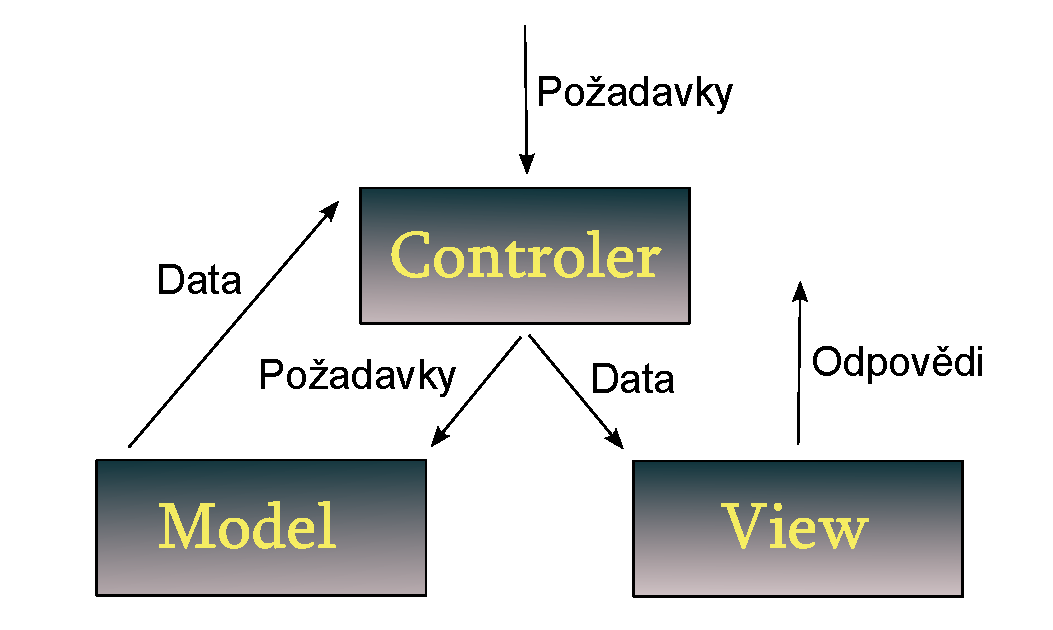
\includegraphics[scale=0.6]{mvc.pdf}
\caption{Architektura MVC}
\end{center}
\end{figure}


Prezentační vrstva je realizována prostřednictvím technologie JSP (Java Servlet Pages), zabezpečení a přihlašování uživatelů pak využívá frameworku Spring Security. Dále je pluginem Sping Social zajištěno prostřednictvím definovaného API propojení webové aplikace se sociálními sítěmi Facebook, Twitter a LinkedIn. Spring Social také slouží ke integraci možnosti přihlašování uživatelů prostřednictvím účtů zmíněných sociálních sítí.

Aplikační vrstva využívá zejména technologií Spring MVC a Spring Core a zajišťuje zpracování veškerých uživatelských požadavků pro ukládání a čtení dat, která získává z datové vrstvy. Persistentní data jsou uložena v relační databázi Oracle 11g, přičemž k jejich zpracování je použito objektově-relační mapování frameworku Hibernate. Ten využívá XML souborů pro mapování tabulek na POJO objekty, jež tvoří perzistentní vrstvu. Framework Hibernate zároveň umožňuje odstínit datovou vrstvu od implementační závislosti na zvolené databázi, jejíž případná obměna by následně nevyžadovala příliš velké zásahy do zdrojových kódů portálu \cite{_16}.


\section{Persistentní data}
\hspace{0.65cm}Databáze Oracle jež slouží ke ukládání persistentních dat uchovává veškeré naměřené hodnoty zaznamenaných experimentů. Tato data mají z pohledu databáze podobu binárních souborů s velikostí řádu desítek až stovek MB. Tato naměřená data by ovšem ztrácela hodnotu, kdyby byla uchovávána jako samostatná. Proto databáze obsahuje další tabulky, jež nesou metadata prováděných experimentů. Kontext experimentu je popsán především hodno-\\tami o prostředí laboratoře a zúčastněných osobami. Prostředí laboratoře je charakterizováno například teplotou, použitým hardwarem a softwarem. Nedílnou součástí popisu experimentu je také scénář zaznamenávající samotný postup měření, který má podobu binárního souboru. Dalšími důležitými daty jsou také informace o použitých elektrodách měřících EEG, u kterých je důležitý jejich typ a poloha. Co se týče osob účastnících se experimentu, zaznamenává se měřící a především měřená osoba. U osob jsou uchovávány osobní a kontaktní údaje a také data nutná pro přihlašování do portálu. Osoby se mohou sdružovat do různých výzkumných skupin, jež nesou seznam svých členů a vlastníka. Podstatným údajem jsou také identifikátory skupin vázané k hodnotám číselníků charakterizující vlastnosti experimentu, které tak napomáhají výzkumníkům zaznamenávat vlastní vybrané předdefinované hodnoty. Další tabulky ještě zaznamenávají historii stahování, zveřejňované články a jejich textové komentáře. Rezervace laboratoře obsahuje údaje o počátečním a koncovém času události a také rezervující osobě. 


\chapter{Relační datový model}
\hspace{0.65cm}Jak již bylo zmíněno v předchozí kapitole, webová aplikace EEG/ERP portál uchovává data v relační databázi – lze na ně tedy pohlížet jako na relační datový model. Vzhledem k tomu, že další část práce se bude zabývat úpravou současného datového modelu portálu, bude vhodné uvést zde základní popis a vlastnosti obecného relačního modelu.

Základem relačního modelu dat, který byl popsán již v roce 1970 je takzvaná relace neboli tabulka \cite{_17}. Z matematického hlediska můžeme {\it n}-ární relaci chápat jako libovolnou podmnožinu kartézského součinu {\it n} množin \cite{_18}. Množinou je zde myšlena doména jednoho konkrétního sloupce tabulky, tedy všechny přípustné hodnoty, kterých může libovolný řádek v daném sloupci tabulky nabývat. V důsledku tedy máme tabulku tvořenou {\it n} sloupci ({\it n}-ární relace) a {\it x} řádky, kde každý řádek reprezentuje jeden prvek z množiny tvořené kartézským součinem {\it n} množin. V případě, že by každá z {\it n} množin byla konečná (řádky daných sloupců mohou nabývat konečného počtu hodnot), bude konečný i kartézský součin těchto množin a tabulka tak může mít jen konečný a tudíž omezený počet neopakujících se řádek (duplicity v tabulce neuvažujeme, neboť by neměly žádný smysl – jednalo by se o redundantní data) \cite{_18}.

Uvedená reprezentace matematického pojmu relace jako databázové tabul-\\ky je základem takzvaného schéma relace. Toto schéma obsahuje název relace, jména všech atributů (sloupců tabulky) a jejich integritních omezení – tedy domény \cite{_19}. Domény jednotlivých atributů jsou v systémech řízení báze dat reprezentovány datovými typy, tedy např. číselný typ, textový řetězec či datum. Tabulku lze tedy chápat jako určitou formu znázornění relace \cite{_21}.
Jedna tabulka slouží zpravidla k uchování údajů o jednom druhu objektů \cite{_20}. \\V případě portálu tak například tabulka {\it Person} uchovává pouze data o osobách – jeden řádek neboli záznam tedy reprezentuje údaje o jednom člověku, které jsou strukturované do sloupců, např. jméno, příjmení, email apod. Názornější představu konkrétní relace je možné získat z obrázku 4.1. Aby bylo možné s daty tabulky pracovat, zavádí se aparát, který zajišťuje jednoznačnou identifikaci každého záznamu - primární klíč. Primární klíč je atribut či skupina atributů, která je pro každý záznam tabulky jedinečná (stejně jako název tabulky v databázi) \cite{_20}. V případě zmíněné tabulky {\it Person} by tak mohl posloužit například atribut email, neboť žádné dvě osoby nemo-\\hou logicky mít stejnou emailovou adresu (což by mělo být zajištěno ze strany 

\begin{figure}[htb]
\begin{center}
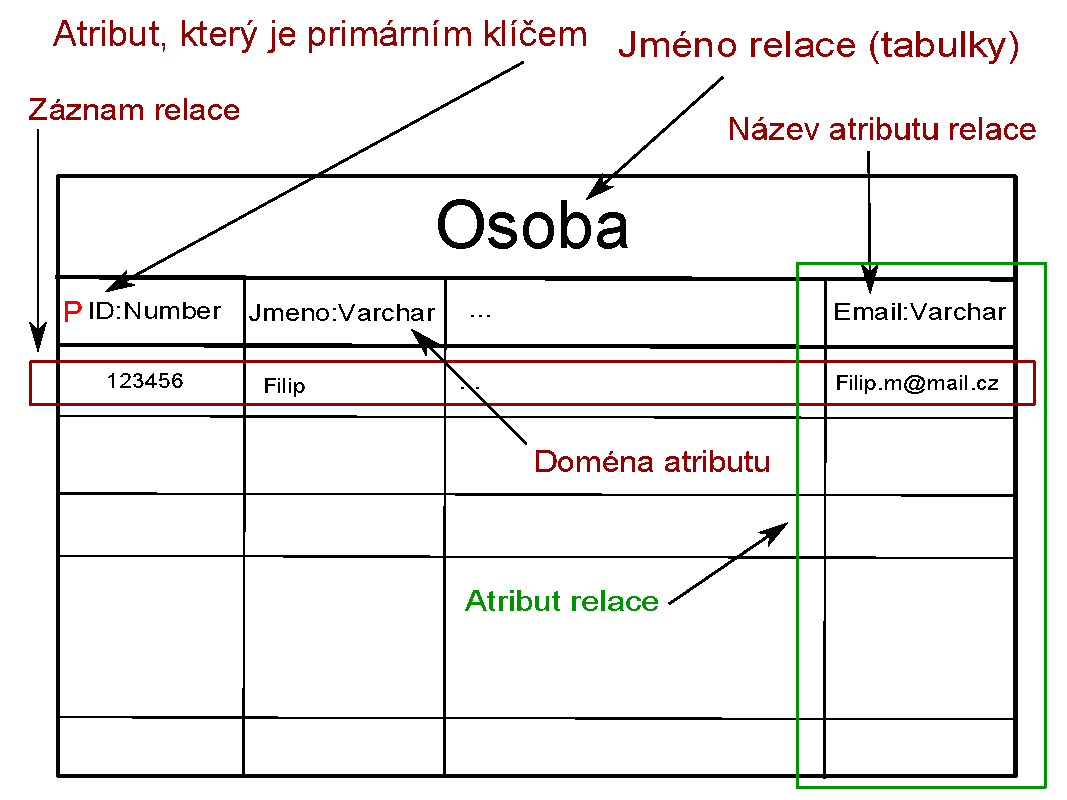
\includegraphics[scale=0.7]{relace.pdf}
\caption{Znázornění relace}
\end{center}
\end{figure}

domény dané emailové adresy). V případě že tabulka neobsahuje žádný atribut, který by potřebnou jedinečnost záznamů zajišťoval, je nutné jej přidat. To je realizováno např. atributem ID, obsahujícím číslo z číselníku, jehož hodnota je inkrementována po každém přidání dalšího záznamu do tabulky {\it Person}. Tento identifikátor položky sice jednoznačně určuje daný záznam v tabulce, nikoliv už však v rámci celé databáze (pokud uvažujeme více tabulek) či vně databáze. V jedné databázi je tedy možné mít například tabulky {\it Person} a {\it Experiment}, jejichž primárními klíči bude atribut s názvem ID typu celého čísla. V takovém případě je pak i možné aby obě tabulky obsahovaly 2 různé záznamy jež budou jednoznačně identifikovatelné stejnou číselnou hodnotou (ale v kontextu dané tabulky). Z toho důvodu je pro jednoznačnou identifikaci záznamu nutné znát jak hodnotu příslušného atributu obalující relace, tak i její název. 


\section{Limity relační databáze}

\subsection{Dědičnost}


\hspace{0.65cm}Relační databáze může samozřejmě obsahovat větší množství tabulek (za předpokladu že mají vzájemně různé názvy). Každá tabulka tak sdružuje záznamy, jejichž obsah si je v určitém smyslu blízký. Z hlediska objektově orientovaného přístupu, který je realizovaný např. nástrojem Hibernate, lze tabulku chápat také jako třídu a její záznamy jako instance dané třídy. Každá takováto instance má pevně daný počet atributů, který je definován obalující třídou. Uvažujme například tabulku {\it Person}, která ponese údaje jak o osobách které jsou cílovým objektem experimentů tak údaje o výzkumných pracovnících. U obou skupin nás budou zajímat společné atributy jako jméno a příjmení, ale některé atributy budou různé. U testovaných osob to bude např. věk, zatímco u výzkumníků např. titul. Uvažujeme-li objektový přístup k takovéto tabulce, můžeme využít dědičnosti. Vytvoříme tedy třídu {\it Person}, která ponese všechny společné atributy a od ní bude zděděna třída pro výzkumníky a třída pro testované osoby. Tyto třídy budou obsahovat atributy, které jsou specifické pro danou skupinu. Z pohledu relačního modelu je tento problém řešitelný obtížněji. Je možné například vytvořit 2 samostatné tabulky pro dané skupiny či ponechat jednu tabulku, která ponese všechny atributy a každá skupina bude mít vyplněna jen jejich část. Podobný problém by vznikl například při potřebě dodat další atribut jen omezenému počtu osob jedné ze skupin. Z uvedeného příkladu je patrné, že dynamické rozšiřování záznamů obsažených v jednotlivých tabulkách je poměrně obtížné.

\subsection{Vztahy mezi relacemi}

\hspace{0.65cm}Relační model dovoluje také zaznamenávat vztahy mezi jednotlivými tabulkami a provazovat tak záznamy z různých tabulek. Tyto vazby se realizují prostřednictvím atributů označovaných jako cizí klíč \cite{_20}. Hodnotou cizího klíče je pak hodnota primárního klíče tabulky, která je cílem vytvářené vazby. Z hlediska kardinality vztahu je možné rozlišit 3 základní případy {\it 1:1} , {\it 1:N} a {\it M:N} \cite{_22}. Vztah {\it 1:1} vyjadřuje případ, ve kterém záznam jedné tabulky odpovídá záznamu jinému tabulky. Tento případ není příliš častý a většinou se řeší umístěním obou záznamů do jediné tabulky. Vztah {\it 1:N} reprezentuje situaci, kdy se jednomu záznamu tabulky přiřazuje více záznamů jiné tabulky. Příkladem takové vazby může být vztah záznamů tabulek {\it Person} a {\it Reservation}. Jedna osoba tedy může mít {\it N} rezervací laboratoře, ale každá rezervace má jako vlastníka právě jednou osobou. V modelu je tato informace realizovaná přidáním atributu {\it person\_id} do tabulky {\it Reservation}. Tento atribut se tak stává cizím klíčem a ponese hodnotu primárního klíče tabulky {\it Person} pro příslušný záznam cílové osoby. Samotná vazba tedy obsahuje informaci o zdrojové záznamu, cílovém záznamu a také název vazby který je reprezentován názvem atributu pro cizí klíč tabulky.

Posledním druhem vazby je vztah {\it M:N}, jež slouží k reprezentaci stavu, kdy {\it M} záznamům jedné tabulky odpovídá {\it N} záznamů jiné tabulky. Tento stav je v relačním modelu řešen rozložením na dvě vazby {\it 1:N} a {\it 1:M}, které jsou pak realizovány vytvořením další tabulky, jejíž záznamy budou obsahovat cizí klíče obou tabulek. Pro realizaci takové vazby je tedy nutné vložit do databáze další tabulku a v případě potřeby rozlišení druhu jednotlivých vazeb je zapotřebí buď dalšího atributu jež by vztah popisoval, či pro každý druh vazby mít vlastní tabulku (což se týká i případu vazby {\it 1:N}). Pokud by ovšem bylo zapotřebí popsat také vztahy mezi jednotlivými vazbami nastává problém, který je řešitelný velmi obtížně \cite{_20}.


\section{Datový model EEG/ERP portálu}
\hspace{0.65cm}Současnou podobu relační databáze portálu tvoří přibližně 80 tabulek. Naměřená data experimentů (hodnoty EEG signálů) jsou uložena v podobě binárních souborů v tabulce {\it DATA\_FILE}, spolu se popisnými údaji jako je název či datový typ mající podobu textového řetězce nebo čísla. Tyto popisné údaje lze označit jako metadata binárního souboru naměřených dat. Metadata scénáře experimentu uložená v tabulce {\it SCENARIO} obsahují popisné informace dalších binárních souborů, jež jsou uloženy v tabulce {\it SCENARIO\_TYPE\_NONXML} obsahující popis průběhu měření. Obě tabulky {\it SCENARIO} a {\it DATA\_FILE} obsahují vazbu na tabulku {\it EXPERIMENT}, která obsahuje buď přímo metadata experimentu (nikoliv však souboru naměřených dat) nebo zajišťuje provázání s jinou tabulkou jež je nese. Z aktuálního modelu je patrné, že jeden experiment je popsán jedním scénářem, ale může obsahovat více (binárních) souborů naměřených dat.

Tabulka {\it EXPERIMENT} s klíčovými metadaty obsahuje také dvě vazby na tabulku {\it PERSON}, jež slouží ke zaznamenání měřené osoby a experimentátora (vlastníka experimentu). Z hlediska datového modelu není mezi těmito osobami rozdíl, neboť jsou všechny uloženy v jediné tabulce a tudíž jsou všechny osoby popsány stejnou množinou atributů. Některé testované osoby například vůbec nemusejí potřebovat přístup do portálu, ale tabulka ve které jsou zaznamenány obsahuje atributy uživatelského jména a hesla (i když mohou nabývat hodnoty NULL). Stejná situace nastává i pro další referencované tabulky {\it ARTICLES}, {\it ARTICLES\_COMMENTS} či {\it RESERVATION}. Datový model tak nikterak nezabraňuje, aby měřené osoby měly své články, přidávaly k nim komentáře nebo rezervovaly laboratoř (vychází se z předpokladu, že portál slouží zejména pro výzkumné pracovníky, nikoli pro testované osoby). 

Obdobná situace nastává v případě tabulky {\it RESEARCH\_GROUP}, sloužící ke sdružování osob do výzkumných skupin. Její vazby na tabulku {\it PERSON} zajišťují, že každá skupina má svůj název, popis a také vlastníka. Každá skupina může mít samozřejmě více členů, což zajišťuje rozkladová tabulka {\it RESEARCH\_GROUP\_MEMBERSHIP}, jež obsahuje i roli člena ve skupině (ve smyslu uživatelský práv). Samotná tabulka ovšem poměrně značně zasahuje do celého datového modelu, díky množství rozkladových tabulek sloužících ke kategorizaci hodnot specifických metadat experimentů ke vybraným skupinám. Díky tomu je možné, aby vybraná skupina mohla definovat pro své potřeby vybrané hodnoty pro určitá metadata – např. pro tabulku {\it HARDWARE} definovat množinu přístrojů, které ke svým výzkumům využívá. Díky rozkla-\\dovým tabulkám může navíc více skupin sdílet stejné hodnoty položek hard-\\waru. Tyto tabulky s dodatečnými metadaty experimentu jako například zmíněný {\it HARDWARE}, {\it SOFTWARE} či {\it WEATHER} sice popisují kontext měření, ale z hlediska datového modelu se jedná pouze o nekategorizovaná data vázaná (často nepřímo) na tabulku {\it EXPERIMENT}. Není tedy možné sdružit některé parametry měření do skupin – např. tabulky {\it PHARMACEUTICAL} a {\it DISEASE} označit jako medicínské parametry s specifikovat tak jednoduchou hierarchickou kategorii metadat experimentů.

Další problém, který řeší současný relační datový model jen částečně je dynamická rozšiřitelnost struktury dat (ve sémantickém smyslu). V průběhu vývoje portálu se postupně zvyšoval počet tabulek nesoucích specifická meta-\\data experimentu a je i nadále rozšiřován. Pro případ vzniku potřeby popisu daného experimentu parametrem, jenž není definován jako atribut tabulky {\it EXPERIMENT} ani jinou samostatnou tabulkou, obsahuje databáze tabulky {\it EXPERIMENT\_OPT\_PARAM\_DEF} a {\it EXPERIMENT\_OPT\_PARAM\_VAL}. Ty umožňují zaznamenat další hodnoty ve tvaru parametr-hodnota a navíc je sdílet pro více skupin. Nevýhodou tohoto řešení je ale absence možnosti přidat danému parametru více klíčů (chceme-li se vyhnout změně tabulky přidáváním dalších atributů), či tyto údaje ještě více řetězit. Obdobná situace však nastává i v případě samostatných tabulek pro konkrétní metadata experimentu. 

Pro bližší představu o současném datovém modelu portálu je možné nahlédnout do přílohy A obsahující ERA model EEG/ERP portálu.







\chapter{Datový model sémantického webu}
\hspace{0.65cm}Předchozí kapitola se zabývala daty, která jsou sdružovaná a reprezentová-\\na prostřednictvím relačního modelu. Stejná data ovšem mohou být také uchována prostřednictvím databáze založené na modelu sémantického webu, jemuž bude věnována tato kapitola. V kapitole sémantického webu byla nastíněna koncepce sémantického webu, včetně reprezentace dat. Reprezentací datového modelu sémantického webu je takzvaný RDF graf, který sestává z libovolného počtu RDF výrazů neboli trojic. Každá trojice je tvořena subjektem, predikátem a objektem, které jsou z pohledu sémantického webu dále nedělitelné \cite{_8}. Jedna trojice tak poskytuje jednu elementární informaci o jednom subjektu. Zda-li má objekt trojice podobu jedinečné konkrétní entity už je určeno tím, jestli je reprezentován URI identifikátorem, či se jedná pouze literál nebo anonymní list (blank node). Odlišná situace nastává u subjektu, který může být buď URI identifikátorem nebo anonymním listem. Reprezentace literálem zde již není možná, neboť by se popírala možnost provazování jednotlivých entit trojic, což je klíčová vlastnost sémantického webu \cite{_9}.

Podstatný rozdíl mezi datovým modelem sémantického webu oproti modelu relačnímu je absence jakýchkoliv tabulek. Struktura dat tak není předem specifikována a je tak možné vytvářet v podstatě objektový model jehož vnitřní uspořádání sice může být na první pohled méně přehledné až chaotické ve srovnání s relační variantou, ale tento model je z hlediska struktury dat samopopisný. Záznamy relační databáze sice nabývají významu díky kontextu tabulky resp. jejích atributů, ale sémantické informace o vzájemném vztahu více záznamů různých tabulek už chybí. V datovém modelu jenž je tvořen systémem provázaných trojic jsou sice elementární informace uložené v jednotlivých tripletech, ty ale získávají další informační hodnotu díky kontextu s nimi provázaných trojic. V důsledku tohoto faktu tak každá neizolovaná elementární informace (trojice) v modelu obsahuje sémantickou informaci o vztahu s ostatními daty. Datový model tak ve výsledku obsahuje jak cíleně uložená data (ve smyslu relační databáze) tak i jejich vzájemný kontext, který navíc vytváří z modelu organizovaný systém.

\section{Dynamičnost modelu}
\hspace{0.65cm}Z výše uvedených informací je patrné, že datový model sémantického webu je oproti relačnímu snáze rozšiřitelný a je tak vhodnější pro uchování dat jejichž struktura je v sémantickém smyslu více heterogenní. Bude-li například potřeba vytvořit databází většího množství osob, které se dále člení na určité skupiny jež se liší sledovanými parametry na úrovni skupin i jednotlivců je v principu možné řešit problém dvěma způsoby. Vytvořením relačního modelu je možné kategorizovat osoby prostřednictvím tabulek respektive jejich  atributů, které ale bude nutné dále rozšiřovat s rostoucím počtem nových odlišných skupin a měnit tak do jisté míry pevnou strukturu dat. V případě řešení prostřednictvím sémantického webu je možné přidávat specifické informace pouze vybraným skupinám či jednotlivcům, aniž by se muselo zasahovat do struktury ostatních dat. Je tak možné organizovat jednotlivé objekty (osoby) do různých i prolínajících se skupin a ty popisovat hromadně nezávisle na ostatních, což je myšlenka dědičnosti.

\section{Dědičnost a hierarchie dat}
\hspace{0.65cm}Jazyk RDFS zavádí do datového modelu sémantického webu základní organizační hierarchii. Uložené objekty je možné kategorizovat do jednotlivých tříd stejně jako vlastnosti a ty pak vzájemně hierarchicky organizovat. Jednot-\\livé objekty tak můžou dědit od svých předků (díky konstrukcím {\it rdfs:range} a {\it rdfs:domain}) určité vlastnosti a na své úrovni je sami dále rozšiřovat. Celý tento princip je možné popsat na jednoduchém příkladu znázorněném na obrázku 5.1. Třída ({\it rdfs:Class}) {\it Person} jež definuje dvě vlastnosti ({\it rdf:Property}) {\it name} a {\it surname} má dva potomky ({\it RDFS:SubclassOf}), jež tyto vlastnosti dědí. Potomek {\it Experimenter} dále rozšiřuje své vlastnosti o atribut {\it Email} a potomek {\it Subject} definuje atribut {\it Age}. Informace, že experimentátor {\it Pavel} (jenž je instancí třídy {\it Experiemtnator}) provádí měření na objektu {\it Martin} je zachycena predikátem ({\it rdf:Property}) {\it Measure}. Inverzní činnost „je měřen“ popisuje vlastnost {\it IsMeasured}, přičemž definice inverzního vztahu dovoluje vyjádřit jazyk OWL.

\begin{figure}[htb]
\begin{center}
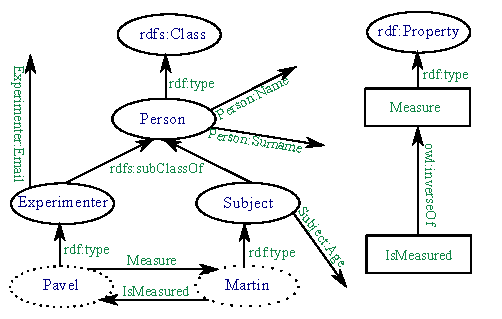
\includegraphics[scale=1.6]{miniportal.pdf}
\caption{Znázornění hierarchické organizace dat}
\end{center}
\end{figure}

\section{Problémy modelu}
\hspace{0.65cm}Jak již bylo zmíněno, tato podoba modelu je výhodná spíše v případech velké různorodosti uchovávaných dat, pro homogenní a z hlediska rozšiřování statická data je stále výhodné řešení využívající tabulek. Sémantický web však slouží především k uchovávání metadat, původní data jež by mohla mít podobu větších binárních souborů by bylo obtížné ukládat tímto způsobem. Technologie a standardy sémantického webu definují datové typy prostřednic-\\tvím schématu jazyka XML, jenž sice připouští také binární typy např. base64Binary, ale pravděpodobně není vhodné je využít pro uložení většího binárního souboru do tohoto datového modelu z důvodu výkonnosti a séman-\\tické využitelnosti v rámci modelu \cite{_27}.


\section{Porovnání modelů}
\hspace{0.65cm}Pro jednoduché porovnání datového modelu sémantického webu a relačního datového modelu poslouží níže uvedená tabulka 5.1, jež srovnává výhody (+) a nevýhody (-) obou modelů.

\begin{table}[htbp!]

\label{značka tabulky}
%\begin{center}
\begin{tabular} { |  m{7.4cm} | >{\centering} m{2.6cm} |  > {\centering} m{2.6cm} | } 
\hline
&  {\bf Relační model} & {\bf Model sémantického webu} \tabularnewline 
\hline
Dědičnost & + & -\tabularnewline
\hline
Dynamická rozšiřitelnost modelu & + & -\tabularnewline
\hline
Typování meziobjektových vazeb & + & -\tabularnewline
\hline
Unifikace idetifikátorů objektů & + & -\tabularnewline
\hline
Hierarchická organizace dat & + & -\tabularnewline
\hline
Sémantika datového modelu & + & -\tabularnewline
\hline
Ukládání rozsáhlých datových objektů & - & +\tabularnewline
\hline
Uchování (sémanticky) homogenních dat & - & +\tabularnewline
\hline
Počet dosptupných nástrojů pro uchování persistentních dat & - & +\tabularnewline
\hline
\end{tabular}

%\end{center}
\caption{Srovnání výhod a nevýhod datových modelů}
\end{table}

\vspace{0.3cm}

Z výše uvedené tabulky je patrné, že vhodnost použití vybraného modelu je odvislá od typu a struktury dat, jež by měl datový model uchovávat. Jednotlivé řádky tak stručně shrnují vhodnost modelu pro vybranou vlastnost uchovávaných dat. Poslední položkou je počet dostupných nástrojů umožňují-\\cích uchování persistentních dat, kterou je míněno množství softwarových řešení databázových úložišť umožnujících uchování dat ve vybrané, modelu přirozené podobě. Pro relační databáze je takových nástrojů poměrně široká řada, ale pro úložiště dat sémantického webu je výběr o poznání menší, navíc mnoho z těchto dostupných nástrojů je spíše experimentálního charakteru. Jejich popisu a výběru se věnuje následující kapitola.


\chapter{Nástroje pro vývoj sémantického webu}
\hspace{0.65cm}Jak již bylo zmíněno v kapitole Sémantický web, jazyk RDF je jedním ze základních stavebních prvků  technologie sémantického webu. Současná podoba tohoto jazyka vychází ze specifikace W3C \cite{_6} z února 2004. Za dobu uběhlou od publikace zmíněné specifikace do současnosti (2013) vznikla poměrně široká sada nástrojů od jednoduchých utilit až po komplexní softwa-\\rová řešení jež umožňují zpracovávat data v jazyce RDF resp. OWL. Rozsáhlý a vcelku přehledný seznam těchto nástrojů (k datu vzniku této práce celkem 183) dostupný ze zdroje  \cite{_23} poslouží jako primární seznam pro výběr vhodného nástroje. Pro účely této práce se zaměříme na hledání nástroje jež slouží primárně jako persistentní úložiště RDF dat a zároveň poskytuje veřejné Jena/Sesame API pro  komunikaci a umožňuje dotazování jazykem SPARQL nad daty. Další nutnou podmínkou je, aby nástroj poskytoval hybridní úložiště umožňující uchovávat jak relační data tak data v jazyce sémantického webu (zmíněné požadavky vyplývají z následující kapitoly). Tyto poměrně náročné podmínky ovšem splňují pouze dva nalezené nástroje, jejichž popis bude následovat.

\section{Virtuoso}
\hspace{0.65cm}Virtuoso je hybridní databázový server umožňující práci nad více datovými modely. Nástroj poskytuje klasickou relační databázi, RDF databázi trojic, XML databázi a také dokumentově orientovanou databázi. Verze aplikace se zpoplatněnou licencí poskytuje oproti GPL licencované variantě navíc virtuální databázi a také replikaci dat. Virtuální databáze umožňuje zastřešit více databázových systémů jediným centrálním se kterým klient komunikuje. Ve výsledku tak umožňuje klientovi pracovat s více databázemi, které se mu transparentně jeví jako jediná. Díky tomu je například možné prostřednictvím jediného dotazu získat výsledek ze všech databází najednou. Replikace dat slouží  k zajištění konzistence dat takovým způsobem, kdy při např. dvou databázích slouží hlavní databáze k zachycení aktuálních změn dat, které postupně zasílá vedlejší databázi jež obsahuje původní data. Díky tomu obsahuje vedlejší databáze stále konzistentní data neboť při nezdařeném zápisu aktualizace může zažádat hlavní databázi o jejich opětovné zaslání. 

Databázový server poskytuje grafické webové rozhraní, které slouží ke komplexní administraci a také je možné jeho prostřednictvím zadávat libovolné SQL/SPARQL dotazy. Virtuoso implementuje nad relační databází engine poskytující funkcionalitu v podobě standardu SQL-92, podporu pro pohledy, standardní datové typy, procedury, kurzory a také transakce. SPARQL dotazy je možné zadávat stejnými prostředky jako SQL dotazy, či je dokonce vnořovat do SQL dotazů. Díky tomu je možné pracovat s relačním modelem dat a RDF modelem zároveň. Samotné dotazování a další komunikace klientské aplikace se serverem může být realizováno prostřednictvím driverů ODBC/JDBC nebo Java knihovnou poskytující Jena API. Neméně důležitou součásti podpory Java aplikací je i distribuce knihoven pro Hibernate (Hibernate driver a Hibernate dialect). Virtuoso také podporuje import souborů s RDF daty ve formátu N3, Turtle a také nejběžnější RDF/XML \cite{_24}.


\section{Oracle 11g - Oracle Spatial}
\hspace{0.65cm}Oracle Spatial je rozšířením databázového systému Oracle, jež je primárně určeno pro zpracování geoprostorových dat \cite{_25}. Toto rozšíření s sebou ovšem přináší také podporu pro sémantické technologie, která je klíčová pro tuto práci. Standardní instalace Oracle 11g release 2 (současná databáze EEG/ERP portálu), ani žádná z předchozích verzí tuto podporu standardně po instalaci neposkytuje. Její zapnutí je ale pouze záležitostí spuštění instalačního skriptu a následného vygenerování tabulkového prostoru pro systémové tabulky a všechna následně ukládaná data. V tomto tabulkové prostoru je již možné vytvořit sémantickou síť, která ponese všechny systémové RDF tabulky a pohledy, jež jsou nezbytné pro provádění SPARQL dotazů. Při práci s databází je zapotřebí mít k dispozici datový model, který ponese všechny RDF trojice, jež budou vytvářeny. Tento model bude vázán na tabulku, která ponese všechny vytvářené trojice. Do tohoto modelu je již možné zapsat první trojici \cite{_26}.
Pro názornost jednoduchosti tohoto procesu bude uvede výše popsaný postup v podobě SQL příkazů \cite{_26}. 

\begin{verbatim}
1.  ?/md/admin/catsem11i.sql
2.  CREATE TABLESPACE rdf_tblspace DATAFILE 
    '/oradata/orcl/rdf_tblspace.dat' SIZE 1024M AUTOEXTEND 
    ON NEXT 256M MAXSIZE 16384M;
3.  EXECUTE SEM_APIS.CREATE_SEM_NETWORK('rdf_tblspace');
4.  CREATE TABLE family_rdf_data (id NUMBER, 
    triple SDO_RDF_TRIPLE_S);
5.  execute SEM_APIS.create_sem_model('family', 
   'family_rdf_data', 'triple');
\end{verbatim}

První příkaz instaluje podporu sémantických modelů v databázi. Druhým příkazem je na disku vytvořen sobor, který ponese tabulkový prostor pro sémantickou síť a všechny datové modely. Jeho počáteční velikost je nastavena na 1 GB s možností dalšího zvětšení v případě vyčerpání dané kapacity. V tomto tabulkové prostoru je ve třetím kroku vytvořena sémantická síť, ve které je možné vytvářet jednotlivé datové modely. Ve čtvrtém kroku je vytvořena první tabulka se dvěma sloupci, kde se vyskytuje nový datový typ {\it SDO\_RDF\_TRIPLE}. Jedná se o datový typ trojice ve smyslu RDF, který v sobě obsahuje subjekt, predikát a objekt (dle očekávaného standardu). Posledním příkazem byl vytvořen datový model nad předchozí tabulkou, který poslouží pro ukládání konkrétních trojic. Samotné vkládání trojic je pak poměrně jednoduché, a je možné jej nalézt ve \cite{_26}.

Po instalaci podpory sémantických technologií je již tedy možné využívat databázi Oracle jako úložiště RDF dat. Ve výsledku je tedy k dispozici hybridní databáze pro ukládání dat jak v relační podobě tak ve RDF jazyce. Nad zmíněnými sémantickými daty je možné se dotazovat jazykem SPARQL a to skrze stejné prostředky jako v případě jazyka SQL. V důsledku toho je také možné vytvářet vnořené či jinak kombinované dotazy z obou jazyků, stejně jako tomu bylo u nástroje Virtuoso. K sémantickým datům databáze je možné přistupovat samozřejmě stejnou cestou jako k relačním – tedy prostřednictvím ODBC/JDBC driveru, ale Oracle také dodává driver poskytující standardní Jena API pro Java aplikace. 
Databázový systém podporuje odvozovací pravidla jazyka RDF, RDFS i OWL a od verze Oracle 10g je navíc možné, aby uživatel definoval vlastní odvozovací pravidla. Při vytváření dotazu je pak možné určit jakou množinu odvozovacích pravidel (RDF / RDFS / vlastní pravidla či jejich kombinace) chceme do dotazu zahrnout a ovlivnit tím tak jeho výsledek \cite{_26}.


\section{Jena}
\hspace{0.65cm} Jena je Java framework určený pro vývoj aplikací sémantického webu. Nástroj je vyvíjený od roku 2000 v podobě open source projektu, který je nyní dostupný pod Apache licencí. Framework Jena je distribuovaný jako knihovna jež poskytuje \cite{_28}:

\begin{itemize}
\item API pro zápis a čtení RDF dat ve formátu N3, RDF/XML či N-triples
\item API pro práci s ontologiemi na úrovni jazyků RDFS a OWL
\item Reasoner pro zpracování dat jazyků RDF a OWL
\item Dotazovací engine SPARQL
\item Ukládání RDF dat do databáze
\end{itemize}

Jena poskytuje komplexní API umožňující práci s daty sémantického webu. Veškerá zpracovávaná data jež mají podobu grafu jsou uchovávana prostřednictvím modelu. Framework poskytuje 2 druhy modelů, jež se liší svou expresivitou. Základní model umožňující zpracování dat na úrovni jazyka RDF je vhodný pro data s nízkou úrovní sémantiky. Druhý, ontologický model umožňuje maximální využítí nástroje, neboť poskytuje API pro práci s ontologiemi jazyka OWL. Samotný model je možné uchovávat buď pouze v paměti, přičemž je možné jeho data ukládát i opětovně načítat ze souboru, nebo v databázi, která poskytuje příslušný konektor umožňující využítí Jeny jako API k tomuto úložišti. S daty modelu je možné pracovat objektovým způsobem na úrovni trojic či jejjich částí nebo prostřednictvím vykonávání SPARQL dotazů \cite{_28}.




\chapter{Transformace datového modelu}
\section{Rozdělení datového modelu}
\hspace{0.65cm}V předchozích kapitolách jež se zabývaly datovým modelem sémantického webu a relačním datovým modelem bylo možné získat základní představu o obou možnostech reprezentace dat. Rovněž byly nastíněny některé problémy současného relačního datového modelu portálu, jehož úprava je předmětem této práce. Z výše uvedené tabulky 5.2 je patrné že technologie sémantického webu využité pro reprezentaci datového modelu mají i nevýhody, a to zejména v oblasti ukládání rozsáhlých datových objektů, jež je primárním důvodem pro částečné zachování relačního modelu. V rámci této práce tedy bude navržen datový model EEG/ERP portálu, který bude z jedné části  založený na relační databázi a z druhé části na objektové orientované databázi využívající technologie sémantického webu, bude se tedy jedna o hybridní datový model.

Pro rozdělení datového modelu je nutné určit pravidla, podle kterých bude rozdělení provedeno. K tomu bude využito koncepce sémantického webu, který je určený zejména pro ukládání a zpracování metadat. V současném datovém modelu je tedy nutné odlišit základní data od metadat. Následující rozdělení zároveň umožní vyřešit problém ukládání rozsáhlých datových souborů, neboť právě ty budou označeny jako základní data. Na EEG/ERP portál je možné pohlížet jako na aplikaci poskytující prostředky pro ukládání a zpracování experimentů a zároveň umožňující diskusní činnost uživatelů aplikace. Každý prováděný experiment je z pohledu databáze charakterizován dvěma základní-\\mi objekty – binárním souborem zaznamenávajícím naměřeného hodnoty a souborem scénáře, který určuje postup měření. Diskusní funkcionalita portálu umožňuje uživatelům vytvářet textové příspěvky v podobě článků jež mají charakter rozsáhlejšího textového objektu a k těmto článkům mohou další uživatelé přidávat komentáře stejného datového typu. Popis této funkcionality portálu tak v důsledku umožňuje identifikaci základních dat jejichž úložištěm bude relační databáze. V ERA modelu portálu, jež je uveden v příloze A této práce, jsou zmíněné údaje uchovány v tabulkách v podobě rozsáhlých binárních/textových soborů. V relačním modelu tedy ponecháme uchovaná tato data: 



\begin{itemize}
\item Datové soubory se záznamem experimentu
\item Datové sobory se scénářem popisujícím postup experimentu
\item Text článků publikovaných uživateli portálu
\item Text komentářů publikovaných článků
\end{itemize}

\section{Relační část modelu}
\hspace{0.65cm}Relační část datového modelu bude tvořena čtyřmi tabulkami z nichž každá ponese příslušná data dle výše uvedeného seznamu. Z důvodu jednodu-\\chosti budou názvy tabulek převzaty z původního modelu dle původních tabulek nesoucí tato data. Aby bylo možné jednotlivé tabulkové záznamy jednoznačně identifikovat bude do tabulky přidán sloupec nesoucí tento údaj. Pro zachování  koncepce sémantického webu ve výsledném modelu však nebude tímto identifikátorem pouze postupně inkrementované číslo jako v původním modelu, nýbrž se zavede identifikace prostřednictvím URI. Tímto způsobem dosáhneme jednotné identifikace objektů v celém výsledném datovém modelu, přičemž záznamy relační databáze jednoznačně označené prostřednictvím URI budou dále popisovány v datovém modelu sémantického webu, jež bude sloužit k uchování metadat. Ve výsledku tak zmíněná identifika-\\ce údajů prostřednictvím URI zajisti propojení obou částí cílového datového modelu. ERA model relační části nově vytvářeného modelu na obrázku 7.1 je pak poměrně jednoduchý ve srovnání s původní variantou díky absenci uchování metadat. 

\begin{figure}[htb]
\begin{center}
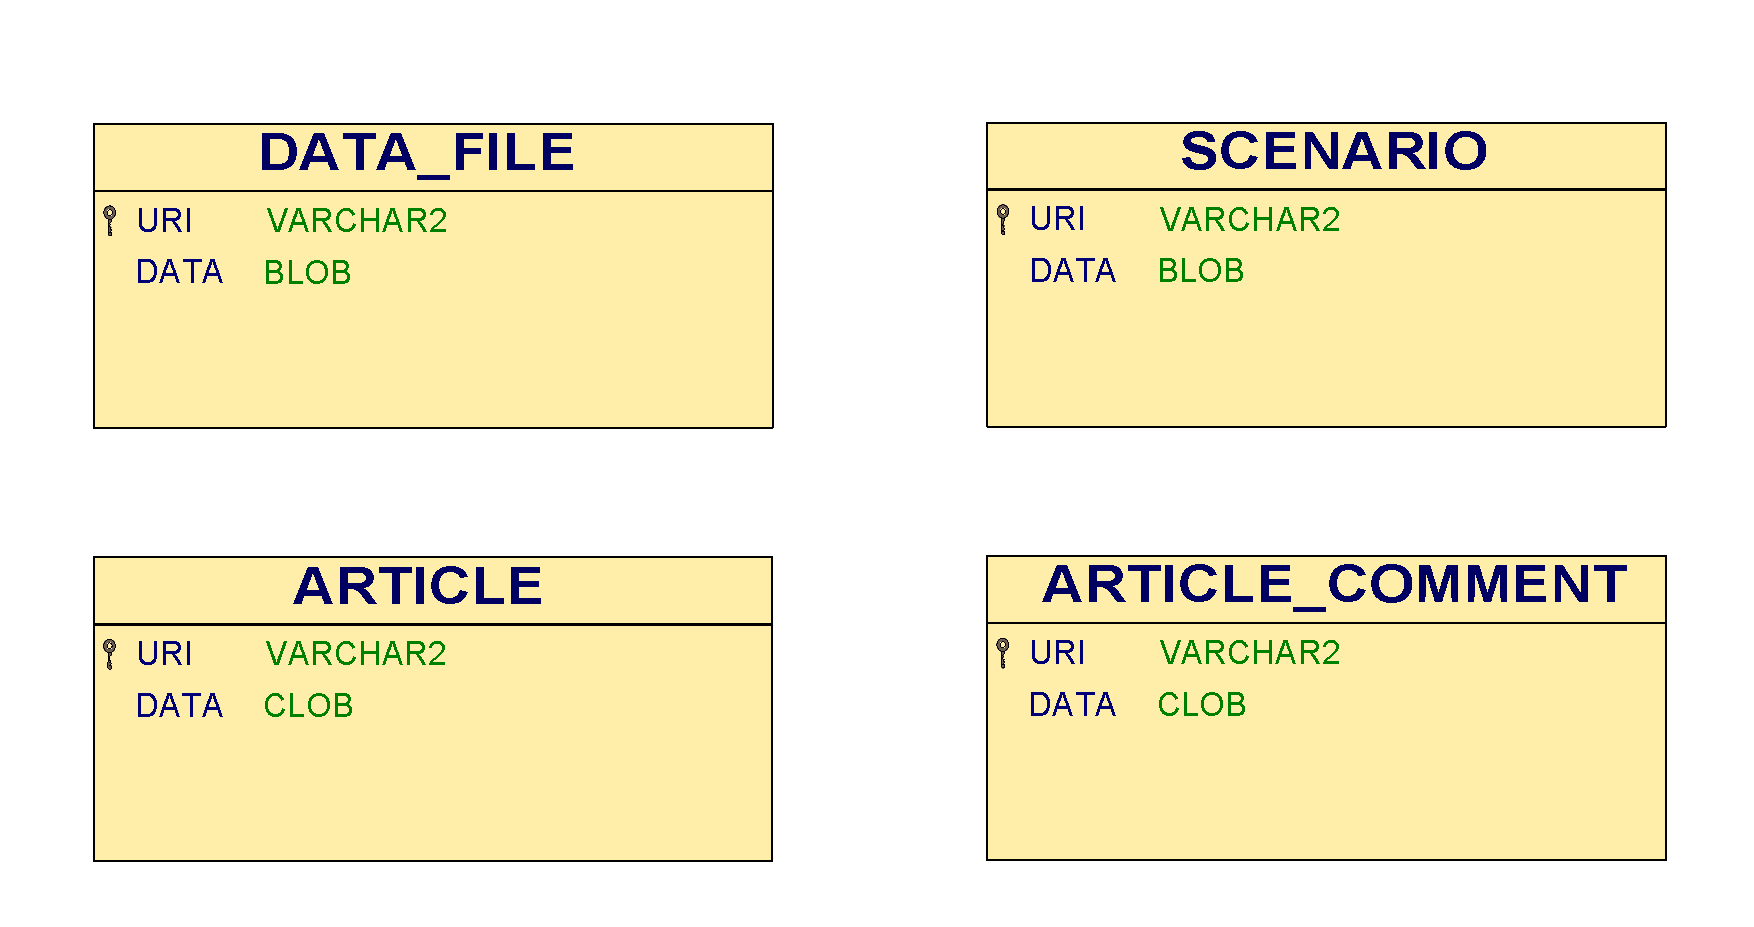
\includegraphics[scale=0.35]{eraNovej.pdf}
\caption{ERA model relační části transformovaného modelu}
\end{center}
\end{figure}


Následující vytvářená sémantická část modelu bude provádět transformaci původního relačního modelu, z jehož tabulek nesoucích zmíněné datové soubory jsou ty atributy odstraněny (z důvodu jejich přesunu do této nové relační části modelu).


\section{Sémantická část}
\hspace{0.65cm}Zbylá část dat původního modelu jež nebude obsažena ve relační části nového modelu je předmětem následující transformace. K jejímu provedení je potřeba nadefinovat obecná pravidla a postup, který by umožňoval transforma-\\ci obecnějšího modelu z důvodu jeho častých změn. I v průběhu tvorby této práce je původní model nadále modifikován a je tak zapotřebí mít k dispozici postup, který by umožnil vytvoření i úpravu nového hybridního modelu tak, aby pokrýval stejnou množinu dat jako původní model v později modifikované verzi. Postup vytvoření nového modelu bude sestávat ze dvou části a to z transformace původních dat do podoby sémantického webu a z dodání sémantiky tomuto modelu, tak aby mohl být do jisté míry samopopisný. 
Pro popis resp. zápis této části modelu budou využity jazyky RDF spolu se RDFS, které dovolují vyjádřit veškerou sémantiku nalezenou v aktuálním modelu.

\subsection{Transformace tabulek}
\hspace{0.65cm}Při transformaci tabulek původního relačního modelu bude využito obdob-\\ného principu jako v případě objektově relačního mapování nástroje Hibernate \cite{_29}. Prvním krokem je identifikace původních tabulek, které neslouží pro rozložení vazby M:N mezi jinými tabulkami. Tyto tabulky budou v nově vznikajícím modelu představovat třídy a záznamy v nich obsažené budou reprezentovány instancemi těchto tříd. To je možné díky jazyku RDFS, který dovoluje vytvářet jednoduchý objektový model složený z tříd a jejich instancí podobně jako např. v jazyce Java. Jednotlivé atributy tabulek pak budou realizovány jako predikáty ({\it rdf:Property}). Transformace struktury původní tabulky prostřednictvím jazyka RDF resp. RDFS se zajistí jazykovými konst-\\rukcemi tak, jak je uvedeno v tabulce 7.1.

Každá takto transformovaná tabulka bude reprezentována jedním URI identifikátorem (stejně jako další objekty) a označení, že se jedná o třídu zajistí konstrukce {\it rdfs:Class}. Původní název tabulky bude součásti hodnoty URI. Každý záznam tabulky bude rovněž popsán prostřednictvím URI a jeho náležitost ke třídě (je instancí třídy) popíše trojice, kde subjektem bude URI této instance, predikátem konstrukce {\it rdf:type} a objektem URI cílové třídy. Jednotlivé atributy tabulky se díky konstrukci {\it rdf:Property} stanou predikáty ve vytvářeném modelu a umožní tak vytvářet typovanou vazbu mezi instancemi a hodnotami jejich atributů (literálů) či mezi instancemi navzájem. 

\vspace{0.25cm}

\begin{table}[htbp!]

\label{značka tabulky}
\begin{center}
\begin{tabular} { | >{\centering} m{3.6cm} |  > {\centering} m{3.6cm} | } 
\hline
Tabulka & {\it rdfs:Class} \tabularnewline
\hline
Záznam tabulky & {\it rdf:type} \tabularnewline
\hline
Atribut tabulky & {\it rdf:Property} \tabularnewline
\hline
\end{tabular}

\end{center}
\caption{Transformace strukur tabulky do sémantického webu}
\end{table}

\vspace{0.25cm}

Transformované atributy (predikáty) je zapotřebí navíc svázat se třídami původních tabulek těchto atributů. Toho se docílí díky konstrukci rdfs:domain, která tak de facto určuje doménu těchto predikátů. Tento výraz ale především slouží k definování náležitosti instance ke své třídě, čehož se docílí vytvořením trojice jejímž predikátem bude transformovaný atribut a subjektem zmíněná instance.


\subsection{Transformace rozkladových tabulek}
\hspace{0.65cm}Původní datový model je z velké části tvořen tabulkami jež rozkládají násobnou vazbu M:N jiných tabulek. Tyto tabulky nebudou transformovány do podoby tříd, nýbrž se pouze využijí jejich atributy, které budou přiřazeny k jedné z provázaných tabulek resp. tříd. Sémantický web připouští přiřazení více různých hodnot objektů subjektům pro stejný predikát. Je tedy možné například instanci třídy {\it Weather} přiřadit pro predikát {\it Research\_group} více cílových skupin. Ve výsledku však bude transformován pouze jeden atribut rozkladové tabulky na predikát, jež bude reprezentovat vazbu mezi první z původních provázaných tabulek prostřednictvím konstrukce {\it rdfs:range} a druhou tabulkou prostřednictvím domény predikátu ({\it rdfs:domain}). Výraz {\it rdfs:range} přiřazený k vybranému predikátu umožňuje vyjádřit náležitost instance ke rodičovské třídě (definované hodnotou {\it rdfs:range}) pokud je tato instance objektem trojice se zmíněným predikátem. V rámci této transformace bude využito {\it rdfs:range} zároveň k vyjádření cílového objektu pro predikát, stejně jako bylo využito domény pro určení zdrojového subjektu daného predikátu. 
Rozhodnutí která z vázaných tabulek určí predikátu hodnotu {\it rdfs:domain} či {\it rdfs:range} je odvislá od sémantického významu této vazby jež bude propojovat výsledné instance tříd a určí tak směr vazby (v případě reprezentace modelu orientovaným grafem se bude určovat směr šipky daného predikátu – viz predikát {\it Measure} na obrázku 5.1).

Pro názornost tohoto postupu bude uvedena ukázka transformace původní tabulky {\it COEXPERIMENTER\_REL} nesoucí atributy {\it EXPERIMENT\_ID} a {\it PERSON\_ID}, tak jak ukazuje obrázek 7.2.


\begin{figure}[htb]
\begin{center}
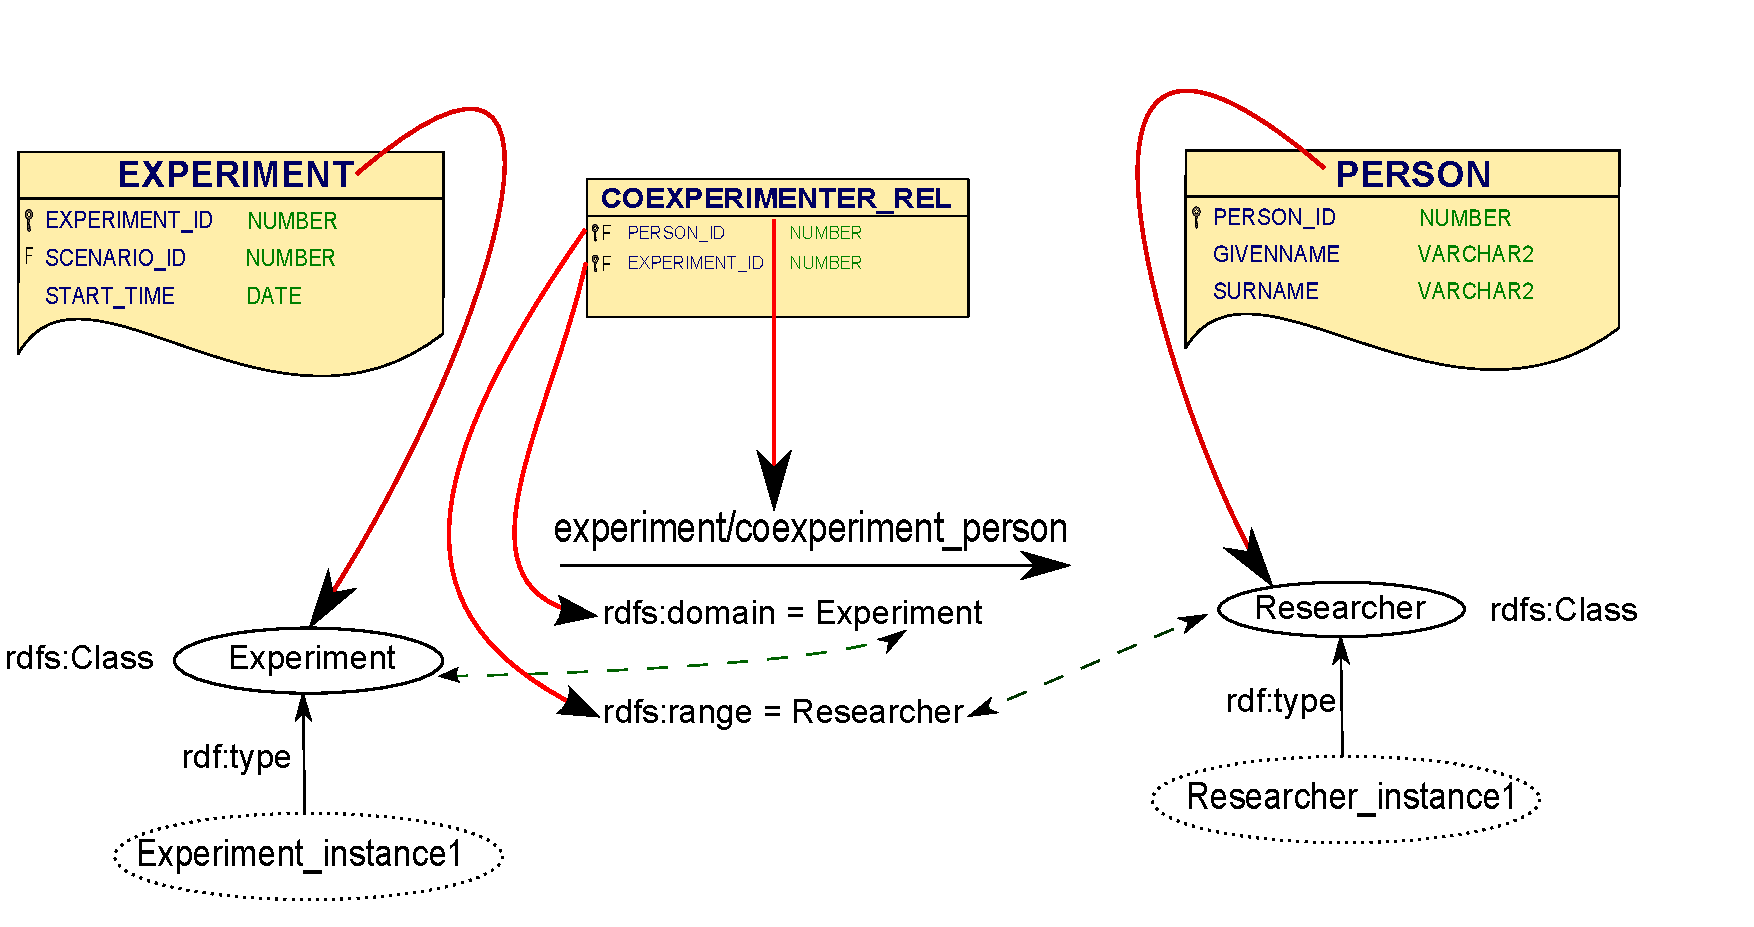
\includegraphics[scale=0.5]{rozkladovka.pdf}
\caption{Znázornění transformace rozkladové tabulky}
\end{center}
\end{figure}


Tato tabulka umožňuje zaznamenat násobnou vazbu mezi záznamy tabulek {\it EXPERIMENT} a {\it PERSON} vyjadřující účast více výzkumníků podílejících se na provádění experimentu. Výsledkem aplikace výše uvedeného postupu bude vzniklý predikát jehož doména ({\it rdfs:domain}) bude mít hodnotu {\it Experiment} (třída) a {\it rdfs:range} hodnotu {\it Researcher}. Hodnotu URI tohoto predikátu lze zvolit např. {\it experiment/coexperiment\_person}.


\subsection{Transformace atributů tabulek}
\hspace{0.65cm}Transformace atributů tabulek již byla popsána v předchozích odstavcích, ze kterých je zřejmý postup vzniku výsledného predikátu. K již uvedenému postupu určení domény predikátu dle tabulky původního modelu je nutné ještě uvést postup určení rozsahu ({\it rdfs:range}) cílových objektů predikátem vázaných trojic. V případě atributů rozkladových tabulek je tento cílový rozsah určen právě jedním z těchto atributů. Rozsah ({\it rdfs:range})  transformova-\\ného atributu u nerozkladové tabulky je určen doménou (ve smyslu relační databáze) tohoto atributu. Pokud je tato (relační) doména původního atributu určena cizím klíčem jiné tabulky s níž má atribut zajistit provázání, pak tato cílová tabulka (transformovaná na třídu) určuje i rozsah predikátu. V opačném případě kdy relační doména je určena pouze datovým typem omezujícím přípustné hodnoty atributu bude rozsah určen rovněž datovým typem, který ale bude definován prostřednictvím XSD datových typů. Určení toho typu je dáno tabulkou XX uvedenou v následující podkapitole.

\subsection{Transformace datových typů}
\hspace{0.65cm}Pro určení datových typů rozsahů ({\it rdfs:range}) predikátů a literálů transfor-\\movaných z hodnot atributů záznamů tabulek slouží následující tabulka 7.2. Ta popisuje transformaci datových typů relační databáze na základní datové typy sémantického webu definované XSD schématem.

\vspace{0.25cm}

\begin{table}[htbp!]

\label{značka tabulky}
\begin{center}
\begin{tabular} { | >{\centering} m{3.8cm} |  > {\centering} m{3.8cm} | } 
\hline
{\bf Relační databáze} & {\bf Sémantický web} \tabularnewline 
\hline
\hline
{\it VARCHAR2} & {\it xsd:string} \tabularnewline
\hline
{\it CHAR} & {\it xsd:string} \tabularnewline
\hline
{\it NUMBER} & {\it xsd:integer} \tabularnewline
\hline
{\it LONG} & {\it xsd:long} \tabularnewline
\hline
{\it FLOAT} & {\it xsd:float} \tabularnewline
\hline
{\it DATE} & {\it xsd:date} \tabularnewline
\hline
{\it TIMESTAMP} & {\it xsd:dateTime} \tabularnewline
\hline
\end{tabular}

\end{center}
\caption{Transformace datových typů relační databáze}
\end{table}

\vspace{0.25cm}

Názvy datových typů relační databáze vycházejí z názvů užívaných portálovou databází Oracle.

\subsection{Transformace záznamů tabulek}
\hspace{0.65cm}Záznamy tabulek původního modelu se transformují na instance tříd ({\it rdf:type}) vzniklých z těchto tabulek. Pro každý záznam se tak vytvoří nové URI jež bude sloužit k jeho identifikaci a především jako subjekt trojic přiřazujících této instanci prostřednictvím vytvořených predikátů hodnoty objektů. Hodnoty těchto objektů závisí na hodnotě atributu původního zázna-\\mu. Bude-li původní hodnota atributu cizím klíčem jiné tabulky pak přiřazova-\\ným objektem bude instance třídy vzniklá ze záznamu určeného tímto cizím klíčem. V opačném případě bude na základě původní hodnoty atributu vytvořen nový literál nesoucí tuto hodnotu, jehož datový typ bude odpovídat transformovanému datovému typu (dle tabulky 7.2) původní domény atributu (původní datový typ atributu).

\subsection{Dodání sémantiky modelu}
\hspace{0.65cm}Nově vytvořenému modelu bude dodána sémantika prostřednictvím hierar-\\chického uspořádání všech transformací získaných tříd a predikátů ke kterým budou navíc dodány popisné informace. Hierarchického uspořádání je možné dosáhnout využitím konstrukcí {\it rdfs:subClassOf} a {\it rdfs:subPropertyOf}. Z původ-\\ního relačního modelu tvořeného množinou rovnocenných tabulek tak vzniká objektový model, který bude mít částečně stromovou strukturu. Jednoduchým způsobem je tedy dosaženo například oddělení zaznamenávaných osob jež provádějí experimenty od těch co jsou měřeným subjektem, tak jak znázorňuje obrázek 7.3.


\begin{figure}[htb]
\begin{center}
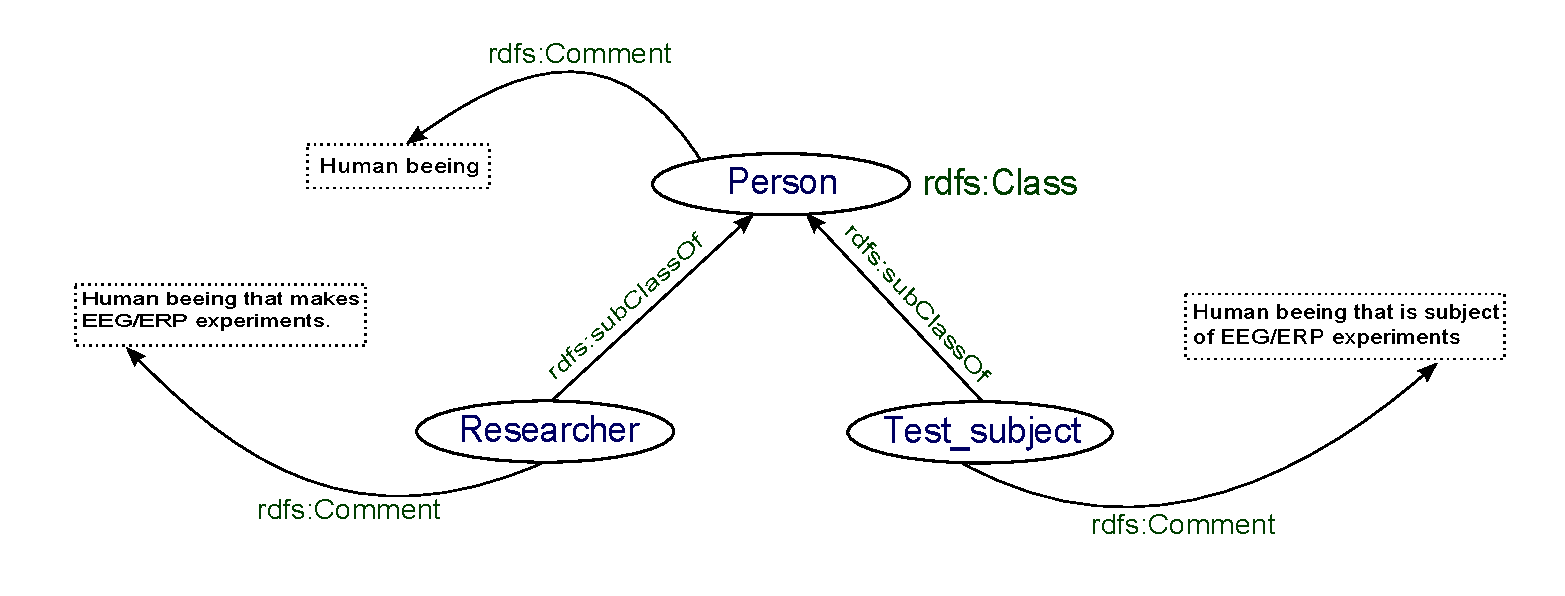
\includegraphics[scale=0.52]{semantika.pdf}
\caption{Znázornění dodání sémantiky modelu}
\end{center}
\end{figure}

Ve výsledném modelu byla dále vytvořena rodičovská třída pro všechny třídy uchovávající údaje o měřících elektrodách či pro metadata popisující scénář měření. Kompletní navržená struktura tříd modelu v XML zápisu ke zobrazena v příloze XX. Význam tohoto zápisu je popsán v následující podkapitole Implementace transformace modelu.

Každé vytvořené třídě a predikátu (property) je navíc dodávána prostřed-\\nictvím konstrukce {\it rdfs:comment} popisná informace (viz obrázek 7.3) umožň-\\ující uživateli získat představu o významu daných struktur modelu, které jsou jinak popsány pouze prostřednictvím URI (byť se sebelépe zvolenou hodnotou). V důsledku tak získáváme do určité míry samopopisný datový model.

\subsection{Řešení rozšiřujících tabulek}
\hspace{0.65cm}Původní relační model obsahuje několik tabulek nesoucích ve svém názvu řetězec {\it PARAM\_DEF} a {\it PARAM\_VAL} jež slouží k uložení dalších rozšiřujících hodnot tabulek ke kterým jsou vázané. Do popisované transformace nebudou tyto tabulky zahrnuty neboť by obsahem svých záznamu porušovaly návrh výsledného modelu. Funkce kterou tyto tabulky v původnímu modelu plní pouze pro vázané tabulky ale poskytuje výsledný transformovaný model všem uloženým datům, díky své koncepci. Toho je dosaženo prostřednictvím možnosti vytváření nových predikátů (property) modelu, které umožňují dodávat další nová metadata libovolným subjektů aniž by došlo k porušení původní struktury modelu. V případě požadavku vícenásobného využití nově definovaných metadat a jejich hodnot je rovněž možné rozšířit model o další třídy a její instance čímž lze dále jednoduše dynamicky datový model rozšiřovat. Názornou ukázkou ověřující toto tvrzení je testovací aplikace popisovaná v následující kapitole testování. 

\subsection{Ukázka transformace}
\hspace{0.65cm}Níže uvedený obrázek 7.4 graficky znázorňuje výsledek provedené transfor-\\mace dle popisovaných pravidel. Vzhledem k velikosti datového modelu je zde zobrazena pouze jeho část, přičemž celý model zapsaný prostřednictvím XML souboru je uložen na přiloženém CD.


\begin{figure}[htb]
\begin{center}
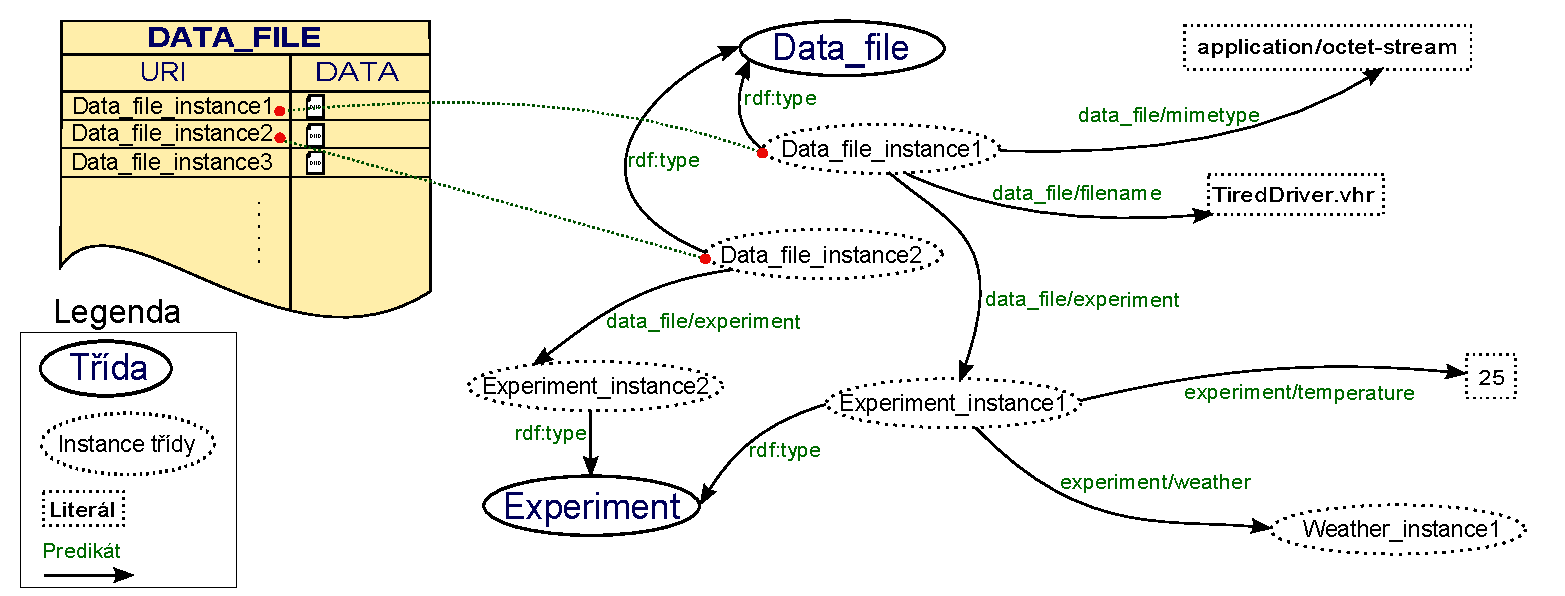
\includegraphics[scale=0.52]{vysledne.pdf}
\caption{Znázornění částí výsledného modelu}
\end{center}
\end{figure}


\subsection{Výhody navrženého modelu}

\begin{itemize}
\item Zápis významu objektů je přímou součásti modelu
\item Jednoduché anotování dat bez změny struktury modelu
\item Dynamicky rozšiřitelný model
\item Možnost libovolných meziobjektových  vazeb
\item Typování meziobjektových vazeb
\end{itemize}


\subsection{Nevýhody navrženého modelu}

\begin{itemize}
\item Datový model rozdělen do dvou částí
\item Ztráta restriktivních omezení z původního relačního modelu
\item Možná ztráta přehlednosti modelu neuváženým rozšiřováním
\end{itemize}

Navržený model poskytuje poměrně širokou řadu výhod, díky které je možné ukládat data způsobem bližším lidskému myšlení. Zásadní nevýhodou modelu je ztráta restriktivních omezení, neboť není možné vynutit na úrovni modelu povinné údaje jako je např. u osob výzkumníků uživatelské jméno či heslo, bez kterých nemohou provést přihlášení do systému a dále jej využívat. Souvisejícím problémem je ztráta možnosti omezení počtu vazeb mezi instancemi tříd, není tak možné například omezit vazbu M:N na 1:1. Všechny tyto záležitosti je nutné řešit v datové vrstvě aplikace pracující s modelem. V rámci tohoto hodnocení navrženého modelu se vybízí také otázka jeho výkonnosti, která bude řešena v kapitole testování.


\chapter{Implementace navrženého modelu}

\section{Formální zápis modelu}
\hspace{0.65cm}V předchozí kapitole byla navržena struktura nového datového modelu portálu, která je tvořena relační částí a částí sémantického webu. Aby bylo možné požadovaný model prakticky využít a otestovat, je nutné zajistit jeho konstrukci v databázovém systému. Pro účely této práce bude model vytvořen v databázových systémech Oracle a Virtuoso, které poskytují prostředky pro hybridní datové úložiště. Vzhledem k tomu, že datový model portálu je neustále modifikován z důvodu implementace nových funkcionalit je vhodné, aby bylo možné model vytvářet co nejvíce automaticky a umožnit tak co nejjednodušeji reflektovat změny původního modelu do transformovaného.

Pro zápis navrženého modelu byl zvolen XML formát a z důvodu přehled-\\nosti, snadné uživatelské modifikace, jednoduchého zápisu hierarchických struktur a následného aplikačního zpracování. Pro usnadnění práce uživatele je k dispozici také XSD šablona jež usnadňuje vytváření dokumentu a jeho případnou validaci. XML dokument tedy slouží k zápisu všech modelem požadovaných struktur, čímž jsou tabulky, třídy a predikáty (property).

Dokument musí začínat definicí tabulek, které jsou specifikovány svým jménem a typem dat jež budou ukládat (binární nebo textové soubory). Název tabulky je zvolen shodně s lokálním jménem URI identifikátoru třídy jejíž instance jsou reflektovány ve zmíněné tabulce prostřednictvím URI. Touto volbou názvu se později v testovací aplikaci docílí propojení tabulek s třídami. Element definující tabulku má název {\it data\_table} a jeho atributy {\it name} a {\it type} slouží ke záznamu jména tabulky typu ukládaných dat. Pro názornost je níže uvedena definice všech 4 tabulek relační části transformovaného modelu.

\begin{verbatim}
<data_table name="article" type="text"/>
<data_table name="article_comment" type="text"/>
<data_table name="data_file" type="binary"/>
<data_table name="scenario" type="binary"/>
\end{verbatim}

Po definici tabulek modelu je dále nutné uvést všechny požadované třídy. Ty jsou určeny svými názvy (URI) a popiskem definujícím ontologický význam třídy (viz obrázek 7.3).
Element definující třídu má název {\it class} a atributy {\it name} a {\it description} slouží zápisu jména třídy a jejího popisku. Pro názornost je opět níže uvedena ukázka definice tříd {\it Experiment} a {\it Article}.

\begin{verbatim}
<class name="article" description="Published article."/>    
<class name="experiment" description="EEG/ERP experiment."/>
\end{verbatim}

Po definici všech tříd je možné zavést jejich nepovinný hierarchický systém. Ten se provádí výčtem potomků vybrané třídy a je možné jej libovolně řetězit. Klíčovým elementem označujícím rodičovskou třídu je {\it parent\_class}, jehož tag ohraničuje potomky definované elementem {\it child} s jediným parametrem name pro název třídy. Definice potomků třídy {\it Person} je uvedena níže.

\begin{verbatim}
<parent_class name="person">
        <child name="person/researcher"/>
        <child name="person/test_subject"/>
</parent_class>
\end{verbatim}

Dalším částí dokumentu je definice predikátů (property). Element pro tuto definici má název {\it property} a jeho atributy {\it name}, {\it range}, {\it domain} a {\it description} postupně slouží k určení jeho jména, rozsahu ({\it rdfs:range}), domény ({\it rdfs:domain}) a sémantického popisku. Ukázka použití je uvedena níže.

\begin{verbatim}
<property 
     name="person/researcher/given_name" 
     range="xsd:string" 
     domain="person/researcher" 
     description="Given name."/>

<property 
     name="person/researcher/group_member" 
     range="research_group" 
     domain="person/researcher" 
     description="Group membership."/>
\end{verbatim}

Poslední části dokumentu je definice hierarchie predikátů, jejíž praktické využití je v této práci spíše okrajové, jak je uvedeno v kapitole testování. Definice hierarchického systému je obdobná jako v případě tříd. Rodičovský predikát je uvozen elementem s názvem {\it parent\_property} s atributem {\it name} nesoucím jméno predikátu. Vnořené elementy děděných predikátu jsou opět definovány názvem {\it child} s atributem {\it name} pro jméno potomka. Ukázka zápisu dědičnosti predikátů je uvedena níže.

\begin{verbatim}
<parent_property name="article_property">
        <child name="article/author"/>
        <child name="article/research_group"/>
        <child name="article/title"/>
        <child name="article/time"/>
        <child name="article/subscription"/>
</parent_property>
\end{verbatim}

Všechny uváděné názvy tříd a predikátů resp. jejich rozsahů a domén jsou (a do cílového dokumentu se tak zapisují) jen lokálními částmi názvu URI, jeho prefix se zadává pouze jednou při zápisu modelu z důvodu jednoduchosti a přehlednosti.
Výsledný dokument s navrženým modelem je spolu s XSD šablonou součástí obsahu přiloženého CD.

\section{Konstrukce modelu}
\hspace{0.65cm}Pro navržený model zapsaný prostřednictvím XML dokumentu je nutné vytvořit aplikace, které jej zapíší do databáze a následně poskytnou API, které umožní s modelem pracovat. Tyto aplikace budou vyvíjeny stejně jako EEG/ERP portál v jazyce Java.

\subsection{Knihovna SemWebModelDbConnector}
\hspace{0.65cm}Pro vytvoření modelu v databázovém systému je nejprve nutné zajistit komunikaci, jež dovolí provádět potřebné operace jak s relační částí, tak i se částí sémantického webu této databáze. K tomuto účelu je navržena knihovna, zastřešující tyto operace prostřednictvím metod interface, jež umožňuje trans-\\parentně komunikovat s vybranou databází bez závislosti, zda-li se jedná o databázový systém Oracle či Virtuoso. Tato knihovna poskytuje metody pro připojení a odpojení od systému a zajišťuje aplikaci jež ji využívá přístup k vybranému modelu sémantického webu spolu s připojením k relačnímu modelu. Na obrázku 8.1 je zobrazen UML diagram této jednoduché knihovny jež je dále využita pro testovací aplikaci a nástroj pro konstrukci modelu. Veškeré implementační detaily jsou patrné z komentovaných zdrojových kódů jež jsou součástí přiloženého CD.

\vspace{0.65cm}

\begin{figure}[htb]
\begin{center}
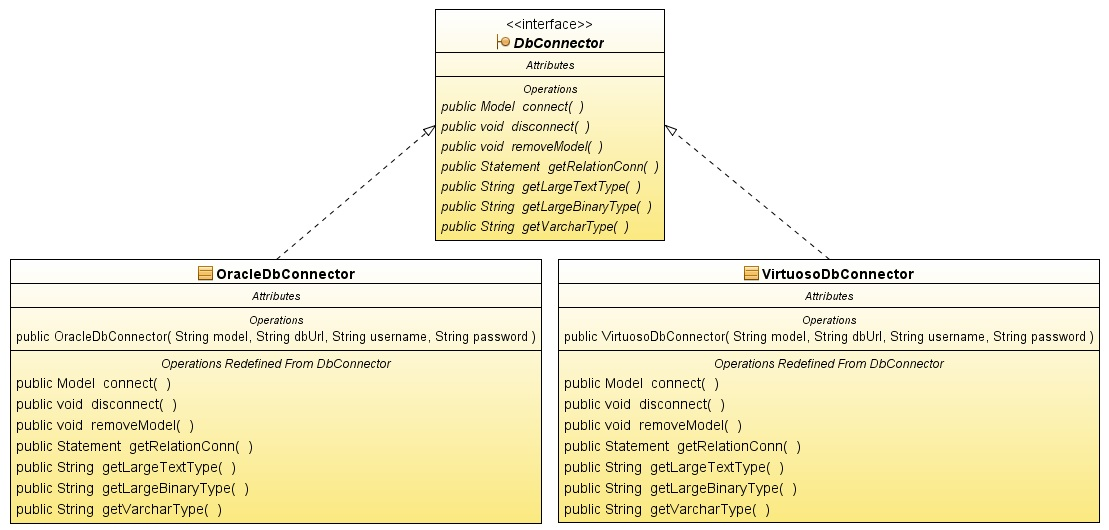
\includegraphics[scale=0.46]{db-connect.jpg}
\caption{UML diagram knihovny SemWebModelDbConnector}
\end{center}
\end{figure}

\subsection{Vytvoření modelu}
\hspace{0.65cm}Za účelem vytvoření cílového navrženého modelu byla implementována aplikace SemWebModelCreator. Ta zajišťuje načítání vstupního XML souboru s modelem a zpřístupňuje tato data aplikaci. Vstupní data jsou načítána ve třídě {\it DataLoader} prostřednictvím SAX parseru \cite{_16}, který na základě získaných hodnot atributů pro dané elementy vytváří datové objekty zastupující požado-\\vané tabulky, třídy a predikáty modelu. K jejich obalení slouží třídy balíku {\it cz.zcu.kiv.eeg.semweb.model.creator.data}. Na základě načtených dat provádí třída {\it ModelCreator} zápis, který sestává z vytvoření obou částí modelů. Nástroj v prvním kroku navazuje prostřednictvím knihovny SemWebModelDbConnec-\\tor spojení s databází, díky čemuž získává přístup k modelu sémantického webu. Pro zápis tříd a predikátů modelu je využito popisovaného nástroje Jena, jenž poskytuje API umožňující ontologický přístup k modelu na úrovni jazyka OWL. Dle načtených dat jsou tak postupně vytvářeny požadované třídy, kterým jsou nastaveny popisné sémantické anotace, a zároveň jsou zařazeny do hierarchického systému prostým nastavením rodičovských tříd či potomků. Predikáty modelu jsou zapisovány obdobným způsobem, přičemž navíc je každému predikátu nastaven definovaný rozsah ({\it rdfs:range}) a doména ({\it rdfs:domain}).

Po dokončení zápisu modelu sémantického webu je přistoupeno k vytváření tabulek relační databáze, což je umožněno díky spojení poskytnutým knihov-\\nou SemWebModelDbConnector při jeho navazování v kroku před zápisem sémantického modelu. Vytváření tabulek je prováděno pouhým vykonáváním SQL příkazů {\it CREATE TABLE} pro všechny požadovaná tabulky lišící se pouze svým názvem a datovým typem atributu {\it DATA} (jež slouží k uchování rozsáhlých datových souborů). 

\subsection{Vytvoření testovacích dat}
\hspace{0.65cm}Aby bylo možné vytvořený model otestovat, je vhodné zajistit i generování testovacích dat. Generování těchto dat zajišťuje třída {\it SimpleDataCreator}, která vytváří pseudonáhodná data v podobě instancí modelem definovaných tříd. Každé instanci jsou navíc přiřazeny hodnoty pro všechny predikáty jež mají doménu shodnou s rodičovskou třídou zmíněné instance. Rozsah generovaných dat je možné specifikovat prostřednictvím celého čísla, které určuje počet generovaných instancí každé třídy.

Pro snadné použití tohoto nástroje má aplikace implementované grafické uživatelské prostředí využitím Java knihovny Swing. Po spuštění aplikace se zobrazí okno dle obrázku 8.2, jež slouží ke specifikaci databázové připojení a nastavení parametrů modelu.


\begin{figure}[htb]
\begin{center}
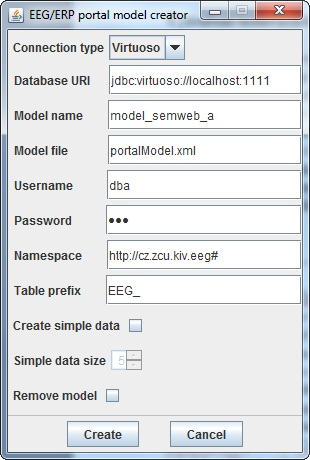
\includegraphics[scale=0.8]{Creator.jpg}
\caption{Okno nástroje pro vytváření modelu}
\end{center}
\end{figure}

Položka {\it ConnectionType} slouží pro výběr cílové databáze modelu (Oracle nebo Virtuoso) jejíž URI je zadáváno v poli {\it Database URI}. Položka {\it Model name} určuje název vytvářeného modelu, jehož popisný XML soubor je zadáván v poli {\it Model file}. Nezbytnou položkou pro spojení s databází jsou uživatelské jméno a heslo v položkách {\it Username} a {\it Password}. Pole {\it Namespace} slouží pro definici URI prefixu všech vytvářených entit modelu, neboť XML soubor popisující model obsahuje pouze lokální části hodnot URI identifikátorů. Poslední pole {\it Table prefix} určuje prefix názvu všech vytvářených tabulek, čímž je později možné v rámci celé relační databáze jednoduše identifikovat tabulky tohoto modelu. 
Zaškrtávací políčko {\it Create simple data} slouží k rozhodnutí, zda generovat testovací data, jejichž velikost určuje položka {\it Simple data size}. Poslední nastavitelná položka je políčko {\it Remove model}, jehož zaškrtnutím bude specifikovaný model smazán namísto jeho vytvoření.
Jednoduchý uživatelský manuál pro použití tohoto nástroje je součásti přílohy XX. Veškeré implementační detaily tohoto nástroje jsou zřejmé z komentova-\\ných zdrojových kódů.


\section{Využití modelu}
\hspace{0.65cm}V rámci zápisu navrženého modelu do hybridní databáze bylo využito API frameworku Jena, který umožňuje jednoduchou práci s konstrukcemi sémantického webu na úrovni jazyka OWL. Pro další praktické využití vznik-\\lého modelu portálu je ovšem toto API příliš jednoduché, neboť neposkytuje metody pro zpracování komplexnějších operací. Z tohoto důvody vznikl požadavek na vytvoření knihovny, která by sloužila jako nadstavba tohoto frameworku a poskytovala API umožňující snáze provádět typické operace datové vrstvy EEG/ERP portálu. 

Implementovaná knihovna SemWebModelApi jež byla vytvořena v rámci této práce poskytuje k cílovému modelu API podobným způsobem jako Jena a umožňuje jednoduchou práci s těmito daty, což je demonstrováno testovací aplikací popsanou v následující kapitole. Operace nad modelem dostupné prostřednictvím API navržené knihovny budou kategoricky rozdělené a popsa-\\né v následujících odstavcích.



\subsection{Operace čtení}
\hspace{0.65cm}Knihovna SemWebModelApi poskytuje přístup k datovému modelu prost-\\řednictvím metod třídy {\it PortalModel}. Operace čtení realizované implemento-\\vanými metodami umožňují práci se třídami, jejich instancemi a s predikáty. Pro získání tříd modelu slouží metody {\it listParentClasses} a {\it listSubClasses}, které umožňují získat URI identifikátory jednotlivých tříd a vytvořit na jejich základě hierarchický strom. Ten může později sloužit jako vstupní bod modelu, který bude poskytovat základní navigaci pro přístup k dalším objektům, kterými jsou především instance tříd, dle konvencí Jeny označované jako „{\it Individual}“. Pro přístup k těmto instancím slouží především metoda {\it listClassInstances}, která vrací potomky třídy předané prostřednictvím jejího URI. Tato metoda vrací list instancí třídy {\it Item}, sloužící jako obalující prvek objektů modelu. Tato abstraktní třída má dva potomky {\it LiteralItem} obalující literály modelu a {\it UriItem}, jež umožňuje nést instanci třídy, případě predikát. Každá instance třídy {\it UriItem} nese URI obalovaného objektu a umožňuje svými metodami získávat další prvky vázané na tento objekt. To je klíčová vlastnost knihovny, která umožňuje s  modelem pracovat v souladu s principy sémantického webu, neboť je možné pro vybranou instanci třídy získat její predikáty vázané objekty, které jsou opět předávané jako instance třídy {\it UriItem} (pokud není cílovým objektem literál). V důsledku je tak možné prostřednictvím jediného subjektu procházet postupně model a získávat požadované informace včetně koncových cílových literálů. Ty jsou reprezento-\\vány instancemi třídy {\it LiteralItem}, která nese datový typ a příslušnou hodnotu tohoto literálu.

Třída {\it UriItem} disponuje metodami umožňujícími získání seznamu prediká-\\tů vázaných k instanci třídy, díky čemuž je možné pro každý objekt získat informace o jeho dostupných vlastnostech a pouze vybranou vlastnost dále zkoumat bez načítání nepotřebných dat což je možné díky nesené vazbě na model v každé instanci {\it UriItem}. Tento způsob umožňuje získávání vybraných informací o dané instanci třídy. Získání těchto instancí pro vybranou třídu je, jak již bylo zmíněno, možné voláním metody {\it listClassInstances} třídy {\it PortalModel}. Aby nebylo nutné při hledání konkrétní instance provádět prů-\\chod celým listem, je možné nastavit prostřednictvím parametru metody filtr, který bude provádět restrikci položek navráceného listu. 

\subsection{Filtrování}
\hspace{0.65cm}Pro nastavení výběru navracených instancí třídy slouží systém podmínek definující vlastnosti požadovaných objektů. Každý vytvářený filtr je tvořen množinou podmínek v logickém součtu, přičemž každá tato podmínka je tvořena další množinou podmínek v logickém součinu. Ve výsledků je tak možné nastavit libovolnou kombinaci nutných a postačující podmínek filtrová-\\ní. Tato navržená koncepce je patrná z UML diagramu tříd filtrování na obrázku 8.3.

Z tohoto obrázku je patrné, že díky rodičovské třídě {\it Condition} všech ostatních tříd je možné vytvářet i poměrně složitý systém podmínek, neboť každá podmínka může být tvořena množinou (listem) podmínek v logickém součtu či součinu. Výsledná koncová podmínka může být 4 typů, které jsou určená následujícími třídami.

\begin{itemize}
\item {\it \bf HasPropertyCondition} - umožňuje nastavit URI predikátu, na který musí mít dotazovaný 
subjekt vázaný objekt (jakýkoliv), např. podmínka že dotazovaná osoba musí mít nastavenou hodnotu emailové adresy, přičemž tato hodnota může být libovolná

\item {\it \bf HasPropertyLikeCondition} - umožňuje nastavit textový řetězec, který musí být obsažen v URI predikátu svazující tento subjekt s jiným objektem, např. podmínka pro řetězec „name“, že dotazovaná osoba musí mít nastavenou hodnotu nějakého jména, lhostejno zda {\it givenname} či {\it surname}
\item {\it \bf PropertyValEqCondition} - umožňuje nastavit textový řetězec, jehož hodnoty musí nabývat objekt vázaný nastaveným URI predikátu, např. podmínka pro osobu, jejíž příjmení musí nabývat hodnoty {\it Novák}
\item {\it \bf PropertyValLikeCondition} - umožňuje nastavit textový řetězec, jehož hodnota musí být obsažena v textové reprezentaci objektu vázaného nastaveným URI predikátu. např. podmínka pro osobu, jejíž přímení musí obsahovat řetězec {\it Novák}, odpovídající objektům příjmení {\it Novák} i {\it Nováková}
\end{itemize}


\begin{figure}[htb]
\begin{center}
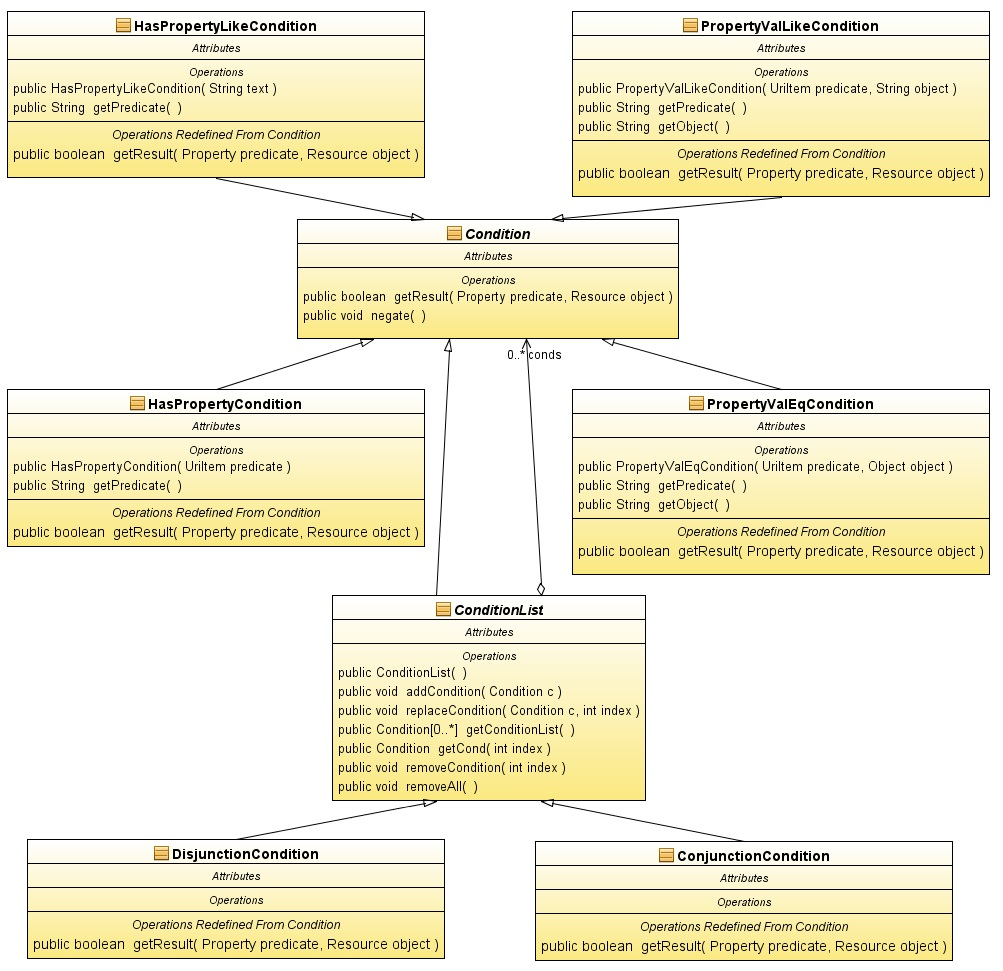
\includegraphics[scale=0.5]{filter.jpg}
\caption{UML diagram tříd filtrování}
\end{center}
\end{figure}


\subsection{Operace zápisu}
\hspace{0.65cm}Zápis nových, resp. aktualizace stávajících dat modelu je možné realizovat opět prostřednictvím metod třídy {\it PortalModel}. Touto cestou je lze vytvářet nové třídy (samostatně či jako potomky stávajících tříd), jejich instance a predikáty (opět s možností hierarchického uspořádání). Aktualizace stávajících hodnot objektů predikátem vázaných ke instancím tříd resp. přidávání nových hodnot je možné realizovat přímo prostřednictvím metod třídy {\it UriItem}, která danou instanci třídy nese. Obdobně lze aktualizovat metodou {\it updateValue} hodnoty existujících literálů ve třídě {\it LiteralItem},  které jsou vytvářeny jako nové hodnoty pro dané vlastnosti (predikáty) instancím tříd prostřednictvím metody {\it addPropertyValue} třídy {\it UriItem}.


\subsection{Operace mazání}
\hspace{0.65cm}Požadavky na mazáni dat modelu lze opět realizovat prostřednictvím metod třídy {\it PortalModel}, jež umožňují odstranění stávajících tříd, jejích instancí a predikátů. Odstraněním stávajícího predikátu dojde ke odstranění všech trojic modelu jež jej obsahují. V důsledku tak všechny instance třídy jež měly nějaký objekt vázaný tímto predikátem o tento údaj přijdou. Odstranění koncových objektů vázaných existujícím predikátem ke instanci třídy je možné realizovat metodou {\it removeValue} třídy {\it LiteralItem} (jedná-li se o literál) nebo přímým odstraněním instance třídy metodou {\it removeIndividual} třídy {\it PortalModel} (jedná-li se o instanci třídy). V tomto případě nedojde k odstraně-\\ní definovaného predikátu z modelu. Poslední mazatelným prvkem modelu jsou třídy, jejichž odstranění zajišťuje metoda {\it removeClasss} třídy {\it PortalModel}. Jejím voláním nad stávající třídou dojde ke odstranění této třídy včetně všech jejích instancí potažmo i trojic vázaných na tyto instance. V důsledku tak odstraněním třídy dojde ke odstranění všech vazeb mezi instancemi nedotčených tříd na mazané instance tříd, neboť jejich odstraněním pozbývají tyto vazby smyslu.

Všechny výše popsané operace jsou patrné z UML diagramu tříd na obrázku 8.4. Detailnější představu o podporovaných operací potažmo imple-\\mentovaných metodách je možné získat z Javadoc dokumentace obsahující podrobný popis všech metod, jejichž názvy jsou významové.


\begin{figure}[htb]
\begin{center}
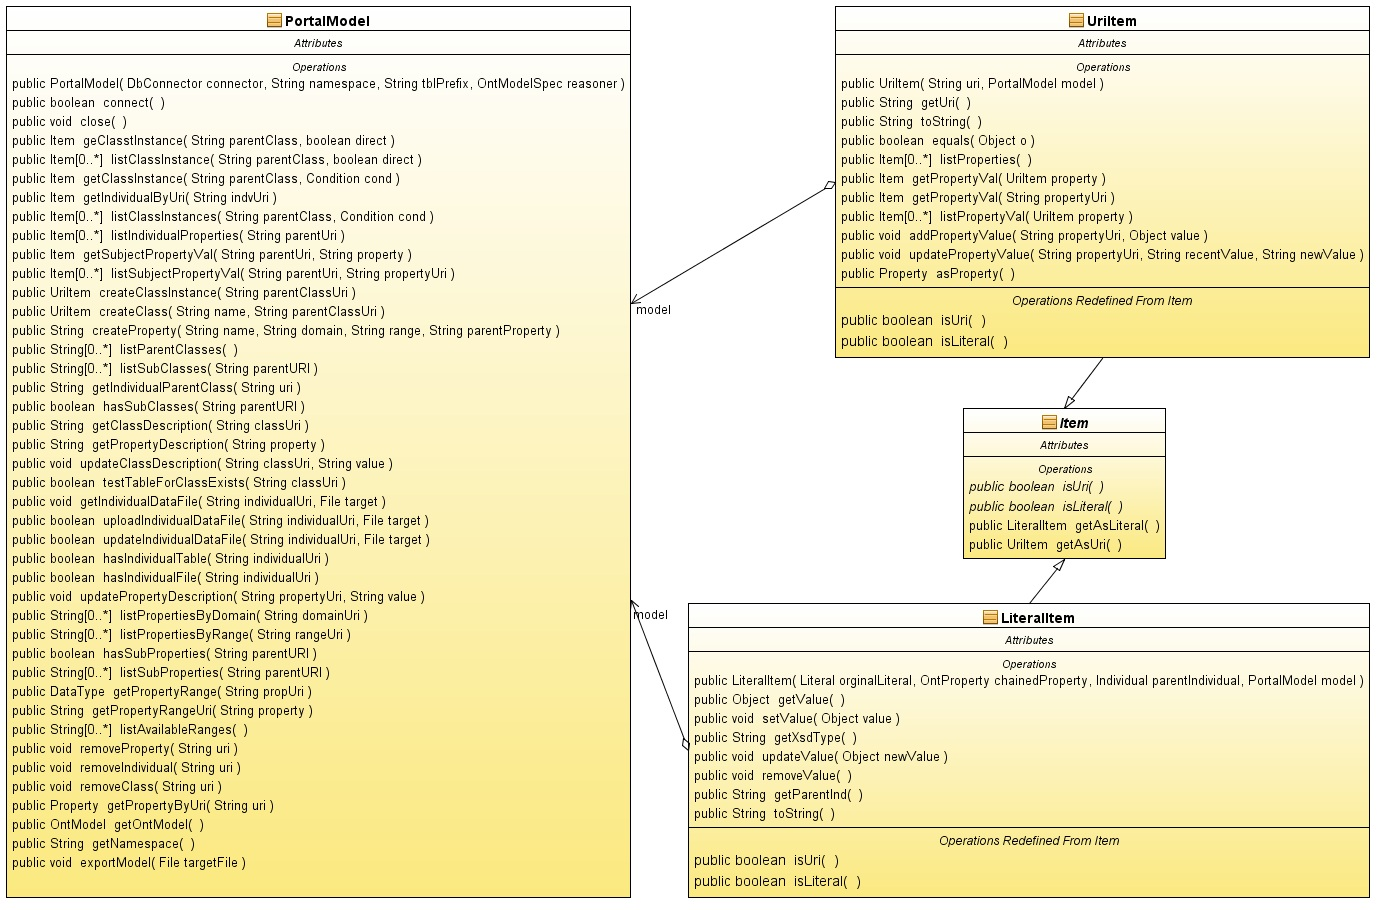
\includegraphics[scale=0.37]{api.jpg}
\caption{UML diagram tříd veřejného API knihovny SemWebModelApi}
\end{center}
\end{figure}


\subsection{Přístup k relačním datům}
\hspace{0.65cm}Pro sjednocený přístup k datům relační části modelu je využito shody názvů (bez definovaného prefixu) relačních tabulek s lokální částí názvu URI příslušných tříd modelu. Název navržené tabulky modelu bez prefixu {\it EEG} má hodnotu {\it DATA\_FILE} stejně jako lokální název třídy {\it data\_file} (nerozlišujeme-li velikost písmen) bez namespace prefixu, čímž je vytvořena pomyslná vazba mezi záznamy tabulky a instancemi třídy {\it data\_file}. Metodami {\it hasIndividual-\\Table} a {\it hasIndividualFile} třídy {\it PortalModel} je pak při dodržení zmíněných konvencí možné zjistit, zda k instancím určité třídy existuje relační tabulka resp. soubory vázáné na konkrétní instance. Tyto soubory je pak možné nahrávat a aktualizovat voláním metod {\it uploadIndividualDataFile} a {\it update-\\IndividualDataFile} třídy {\it PortalModel}. Názorná ukázka tohoto přístupu je realizována testovací aplikací popsanou v následující kapitole.











\chapter{Testování}
\section{Funkční testování}
\section{Výkonnostní testování}
\subsection{Postup testování}
\subsection{Naměřené hodnoty}
\subsection{Diskuze výsledků}


\chapter{Závěr}


\newpage
\thispagestyle{plain}
\noindent
{\bf \LARGE Seznam zkratek a pojmů}\\
%\addcontentsline{toc}{chapter}{Seznam zkratek a pojmů}

\noindent
\begin{description}
\item[API] Application Programming Interface, rozhraní pro programování aplikací
\item[AWT] Abstract Window Toolkit, knihovna Javy pro tvorbu grafického uživa-\\telského rozhraní
\item[EEG] Electroencephalography, metoda vyšetření elektrické aktivity centrál-\\ního nervového
systému
\item[ERP] Event Related Potential, vyšetření reakcí mozku na vnější podněty
\item[OWL] Web Ontology Language, ontologický jazyk sémantického webu
\item[RDF] Resource Description Framework, metodika modelování informací \\v sémantickém webu
\item[SPARQL] SPARQL Protocol and RDF Query Language, dotazovací jazyk nad RDF grafy
\item[URI] Uniform Resource Identifier, jednotný identifikátor zdroje informací
\item[W3C] World Wide Web Consortium, organizace vyvíjející webové standardy
\item[XML] Extensible Markup Language, značkovací jazyk vyvinutý W3C
\item[XSD] XML Schema Definition, XML schéma popisující strukturu XML doku-\\mentu

\item[URI]
\item[Graf]
\item[Orientovaný graf]
\item[XSLT]
\item[MVC]
\item[JSP]
\item[API]


\end{description}


\listoffigures

\bibliography{diplomka}
\bibliographystyle{plain}


\appendix
\newpage


\thispagestyle{plain}

\noindent
{\bf \LARGE Přílohy}
\setcounter{chapter}{1}

\newpage
\thispagestyle{plain}
\section*{{\LARGE A} ERA model databáze EEG/ERP portálu}
\hspace{0.65cm}Priloha A - ERA model portalu
\section*{{\LARGE B} Uživatelský manuál testovací aplikace}
\section*{{\LARGE C} Navržený hierarchický systém tříd modelu}

\end{document}
